% **************************************************************************************************************
% A Classic Thesis Style
% An Homage to The Elements of Typographic Style
%
% Copyright (C) 2012 Andr\'e Miede http://www.miede.de
%
% If you like the style then I would appreciate a postcard. My address 
% can be found in the file ClassicThesis.pdf. A collection of the 
% postcards I received so far is available online at 
% http://postcards.miede.de
%
% License:
% This program is free software; you can redistribute it and/or modify
% it under the terms of the GNU General Public License as published by
% the Free Software Foundation; either version 2 of the License, or
% (at your option) any later version.
%
% This program is distributed in the hope that it will be useful,
% but WITHOUT ANY WARRANTY; without even the implied warranty of
% MERCHANTABILITY or FITNESS FOR A PARTICULAR PURPOSE.  See the
% GNU General Public License for more details.
%
% You should have received a copy of the GNU General Public License
% along with this program; see the file COPYING.  If not, write to
% the Free Software Foundation, Inc., 59 Temple Place - Suite 330,
% Boston, MA 02111-1307, USA.
%
% **************************************************************************************************************
% Note:
%    * You must not use "u etc. in strings/commands that will be spaced out (use \"u or real umlauts instead)
%    * New enumeration (small caps): \begin{aenumerate} \end{aenumerate}
%    * For margin notes: \marginpar or \graffito{}
%    * Do not use bold fonts in this style, it is designed around them
%    * Use tables as in the examples
%    * See classicthesis-preamble.sty for useful commands
% **************************************************************************************************************
% To Do:
%		 * [high] Check this out: http://www.golatex.de/koma-script-warnung-in-verbindung-mit-listings-package-t2058.html
%    * [medium] mathbb in section-titles/chapter-titles => disappears somehow in headlines!!!
% **************************************************************************************************************
\documentclass[ twoside,openright,titlepage,numbers=noenddot,headinclude,%1headlines,% letterpaper a4paper
                footinclude=true,cleardoublepage=empty,abstractoff, % <--- obsolete, remove (todo)
                BCOR=5mm,paper=a4,fontsize=11pt,%11pt,a4paper,%
                ngerman,american,%
                ]{scrreprt}

%********************************************************************
% Note: Make all your adjustments in here
%*******************************************************
% ****************************************************************************************************
% classicthesis-config.tex 
% formerly known as loadpackages.sty, classicthesis-ldpkg.sty, and classicthesis-preamble.sty 
% Use it at the beginning of your ClassicThesis.tex, or as a LaTeX Preamble 
% in your ClassicThesis.{tex,lyx} with % ****************************************************************************************************
% classicthesis-config.tex 
% formerly known as loadpackages.sty, classicthesis-ldpkg.sty, and classicthesis-preamble.sty 
% Use it at the beginning of your ClassicThesis.tex, or as a LaTeX Preamble 
% in your ClassicThesis.{tex,lyx} with % ****************************************************************************************************
% classicthesis-config.tex 
% formerly known as loadpackages.sty, classicthesis-ldpkg.sty, and classicthesis-preamble.sty 
% Use it at the beginning of your ClassicThesis.tex, or as a LaTeX Preamble 
% in your ClassicThesis.{tex,lyx} with \input{classicthesis-config}
% ****************************************************************************************************  
% If you like the classicthesis, then I would appreciate a postcard. 
% My address can be found in the file ClassicThesis.pdf. A collection 
% of the postcards I received so far is available online at 
% http://postcards.miede.de
% ****************************************************************************************************

% ****************************************************************************************************
% 1. Configure classicthesis for your needs here, e.g., remove "drafting" below 
% in order to deactivate the time-stamp on the pages
% ****************************************************************************************************
\PassOptionsToPackage{eulerchapternumbers,listings,drafting,%
				 pdfspacing,%floatperchapter,%linedheaders,%
				 subfig,beramono,eulermath,parts}{classicthesis}										
% ********************************************************************
% Available options for classicthesis.sty 
% (see ClassicThesis.pdf for more information):
% drafting
% parts nochapters linedheaders
% eulerchapternumbers beramono eulermath pdfspacing minionprospacing
% tocaligned dottedtoc manychapters
% listings floatperchapter subfig
% ********************************************************************

% ********************************************************************
% Triggers for this config
% ******************************************************************** 
\usepackage{ifthen}
\newboolean{enable-backrefs} % enable backrefs in the bibliography
\setboolean{enable-backrefs}{false} % true false
% ****************************************************************************************************


% ****************************************************************************************************
% 2. Personal data and user ad-hoc commands
% ****************************************************************************************************
\newcommand{\myTitle}{My Road of 2014\xspace}
\newcommand{\mySubtitle}{Strugling for My Ph.D.\xspace}
\newcommand{\myDegree}{Ph.D.\xspace}
\newcommand{\myName}{Zhiwei Yan \xspace}
\newcommand{\myProf}{Put name here\xspace}
\newcommand{\myOtherProf}{Put name here\xspace}
\newcommand{\mySupervisor}{Put name here\xspace}
\newcommand{\myFaculty}{Put data here\xspace}
\newcommand{\myDepartment}{Put data here\xspace}
\newcommand{\myUni}{Put data here\xspace}
\newcommand{\myLocation}{Darmstadt\xspace}
\newcommand{\myTime}{August 2012\xspace}
\newcommand{\myVersion}{version 4.1\xspace}

% ********************************************************************
% Setup, finetuning, and useful commands
% ********************************************************************
\newcounter{dummy} % necessary for correct hyperlinks (to index, bib, etc.)
\newlength{\abcd} % for ab..z string length calculation
\providecommand{\mLyX}{L\kern-.1667em\lower.25em\hbox{Y}\kern-.125emX\@}
\newcommand{\ie}{i.\,e.}
\newcommand{\Ie}{I.\,e.}
\newcommand{\eg}{e.\,g.}
\newcommand{\Eg}{E.\,g.} 
% ****************************************************************************************************


% ****************************************************************************************************
% 3. Loading some handy packages
% ****************************************************************************************************
% ******************************************************************** 
% Packages with options that might require adjustments
% ******************************************************************** 
\PassOptionsToPackage{latin9}{inputenc}	% latin9 (ISO-8859-9) = latin1+"Euro sign"
 \usepackage{inputenc}				

%\PassOptionsToPackage{ngerman,american}{babel}   % change this to your language(s)
% Spanish languages need extra options in order to work with this template
%\PassOptionsToPackage{spanish,es-lcroman}{babel}
 \usepackage{babel}					

\PassOptionsToPackage{square,numbers}{natbib}
 \usepackage{natbib}				

\PassOptionsToPackage{fleqn}{amsmath}		% math environments and more by the AMS 
 \usepackage{amsmath}

% ******************************************************************** 
% General useful packages
% ******************************************************************** 
\PassOptionsToPackage{T1}{fontenc} % T2A for cyrillics
	\usepackage{fontenc}     
\usepackage{textcomp} % fix warning with missing font shapes
\usepackage{scrhack} % fix warnings when using KOMA with listings package          
\usepackage{xspace} % to get the spacing after macros right  
\usepackage{mparhack} % get marginpar right
\usepackage{fixltx2e} % fixes some LaTeX stuff 
\PassOptionsToPackage{printonlyused,smaller}{acronym}
	\usepackage{acronym} % nice macros for handling all acronyms in the thesis
%\renewcommand*{\acsfont}[1]{\textssc{#1}} % for MinionPro
\renewcommand{\bflabel}[1]{{#1}\hfill} % fix the list of acronyms
% ****************************************************************************************************


% ****************************************************************************************************
% 4. Setup floats: tables, (sub)figures, and captions
% ****************************************************************************************************
\usepackage{tabularx} % better tables
	\setlength{\extrarowheight}{3pt} % increase table row height
\newcommand{\tableheadline}[1]{\multicolumn{1}{c}{\spacedlowsmallcaps{#1}}}
\newcommand{\myfloatalign}{\centering} % to be used with each float for alignment
\usepackage{caption}
\captionsetup{format=hang,font=small}
\usepackage{subfig}  
% ****************************************************************************************************


% ****************************************************************************************************
% 5. Setup code listings
% ****************************************************************************************************
\usepackage{listings} 
%\lstset{emph={trueIndex,root},emphstyle=\color{BlueViolet}}%\underbar} % for special keywords
\lstset{language=[LaTeX]Tex,%C++,
    keywordstyle=\color{RoyalBlue},%\bfseries,
    basicstyle=\small\ttfamily,
    %identifierstyle=\color{NavyBlue},
    commentstyle=\color{Green}\ttfamily,
    stringstyle=\rmfamily,
    numbers=none,%left,%
    numberstyle=\scriptsize,%\tiny
    stepnumber=5,
    numbersep=8pt,
    showstringspaces=false,
    breaklines=true,
    frameround=ftff,
    frame=single,
    belowcaptionskip=.75\baselineskip
    %frame=L
} 
% ****************************************************************************************************    		   


% ****************************************************************************************************
% 6. PDFLaTeX, hyperreferences and citation backreferences
% ****************************************************************************************************
% ********************************************************************
% Using PDFLaTeX
% ********************************************************************
\PassOptionsToPackage{pdftex,hyperfootnotes=false,pdfpagelabels}{hyperref}
	\usepackage{hyperref}  % backref linktocpage pagebackref
\pdfcompresslevel=9
\pdfadjustspacing=1 
\PassOptionsToPackage{pdftex}{graphicx}
	\usepackage{graphicx} 

% ********************************************************************
% Setup the style of the backrefs from the bibliography
% (translate the options to any language you use)
% ********************************************************************
\newcommand{\backrefnotcitedstring}{\relax}%(Not cited.)
\newcommand{\backrefcitedsinglestring}[1]{(Cited on page~#1.)}
\newcommand{\backrefcitedmultistring}[1]{(Cited on pages~#1.)}
\ifthenelse{\boolean{enable-backrefs}}%
{%
		\PassOptionsToPackage{hyperpageref}{backref}
		\usepackage{backref} % to be loaded after hyperref package 
		   \renewcommand{\backreftwosep}{ and~} % separate 2 pages
		   \renewcommand{\backreflastsep}{, and~} % separate last of longer list
		   \renewcommand*{\backref}[1]{}  % disable standard
		   \renewcommand*{\backrefalt}[4]{% detailed backref
		      \ifcase #1 %
		         \backrefnotcitedstring%
		      \or%
		         \backrefcitedsinglestring{#2}%
		      \else%
		         \backrefcitedmultistring{#2}%
		      \fi}%
}{\relax}    

% ********************************************************************
% Hyperreferences
% ********************************************************************
\hypersetup{%
    %draft,	% = no hyperlinking at all (useful in b/w printouts)
    colorlinks=true, linktocpage=true, pdfstartpage=3, pdfstartview=FitV,%
    % uncomment the following line if you want to have black links (e.g., for printing)
    %colorlinks=false, linktocpage=false, pdfborder={0 0 0}, pdfstartpage=3, pdfstartview=FitV,% 
    breaklinks=true, pdfpagemode=UseNone, pageanchor=true, pdfpagemode=UseOutlines,%
    plainpages=false, bookmarksnumbered, bookmarksopen=true, bookmarksopenlevel=1,%
    hypertexnames=true, pdfhighlight=/O,%nesting=true,%frenchlinks,%
    urlcolor=webbrown, linkcolor=RoyalBlue, citecolor=webgreen, %pagecolor=RoyalBlue,%
    %urlcolor=Black, linkcolor=Black, citecolor=Black, %pagecolor=Black,%
    pdftitle={\myTitle},%
    pdfauthor={\textcopyright\ \myName, \myUni, \myFaculty},%
    pdfsubject={},%
    pdfkeywords={},%
    pdfcreator={pdfLaTeX},%
    pdfproducer={LaTeX with hyperref and classicthesis}%
}   

% ********************************************************************
% Setup autoreferences
% ********************************************************************
% There are some issues regarding autorefnames
% http://www.ureader.de/msg/136221647.aspx
% http://www.tex.ac.uk/cgi-bin/texfaq2html?label=latexwords
% you have to redefine the makros for the 
% language you use, e.g., american, ngerman
% (as chosen when loading babel/AtBeginDocument)
% ********************************************************************
\makeatletter
\@ifpackageloaded{babel}%
    {%
       \addto\extrasamerican{%
					\renewcommand*{\figureautorefname}{Figure}%
					\renewcommand*{\tableautorefname}{Table}%
					\renewcommand*{\partautorefname}{Part}%
					\renewcommand*{\chapterautorefname}{Chapter}%
					\renewcommand*{\sectionautorefname}{Section}%
					\renewcommand*{\subsectionautorefname}{Section}%
					\renewcommand*{\subsubsectionautorefname}{Section}% 	
				}%
       \addto\extrasngerman{% 
					\renewcommand*{\paragraphautorefname}{Absatz}%
					\renewcommand*{\subparagraphautorefname}{Unterabsatz}%
					\renewcommand*{\footnoteautorefname}{Fu\"snote}%
					\renewcommand*{\FancyVerbLineautorefname}{Zeile}%
					\renewcommand*{\theoremautorefname}{Theorem}%
					\renewcommand*{\appendixautorefname}{Anhang}%
					\renewcommand*{\equationautorefname}{Gleichung}%        
					\renewcommand*{\itemautorefname}{Punkt}%
				}%	
			% Fix to getting autorefs for subfigures right (thanks to Belinda Vogt for changing the definition)
			\providecommand{\subfigureautorefname}{\figureautorefname}%  			
    }{\relax}
\makeatother


% ****************************************************************************************************
% 7. Last calls before the bar closes
% ****************************************************************************************************
% ********************************************************************
% Development Stuff
% ********************************************************************
\listfiles
%\PassOptionsToPackage{l2tabu,orthodox,abort}{nag}
%	\usepackage{nag}
%\PassOptionsToPackage{warning, all}{onlyamsmath}
%	\usepackage{onlyamsmath}

% ********************************************************************
% Last, but not least...
% ********************************************************************
\usepackage{classicthesis} 
% ****************************************************************************************************


% ****************************************************************************************************
% 8. Further adjustments (experimental)
% ****************************************************************************************************
% ********************************************************************
% Changing the text area
% ********************************************************************
%\linespread{1.05} % a bit more for Palatino
%\areaset[current]{312pt}{761pt} % 686 (factor 2.2) + 33 head + 42 head \the\footskip
%\setlength{\marginparwidth}{7em}%
%\setlength{\marginparsep}{2em}%

% ********************************************************************
% Using different fonts
% ********************************************************************
%\usepackage[oldstylenums]{kpfonts} % oldstyle notextcomp
%\usepackage[osf]{libertine}
%\usepackage{hfoldsty} % Computer Modern with osf
%\usepackage[light,condensed,math]{iwona}
%\renewcommand{\sfdefault}{iwona}
%\usepackage{lmodern} % <-- no osf support :-(
%\usepackage[urw-garamond]{mathdesign} <-- no osf support :-(
% ****************************************************************************************************

% ****************************************************************************************************  
% If you like the classicthesis, then I would appreciate a postcard. 
% My address can be found in the file ClassicThesis.pdf. A collection 
% of the postcards I received so far is available online at 
% http://postcards.miede.de
% ****************************************************************************************************

% ****************************************************************************************************
% 1. Configure classicthesis for your needs here, e.g., remove "drafting" below 
% in order to deactivate the time-stamp on the pages
% ****************************************************************************************************
\PassOptionsToPackage{eulerchapternumbers,listings,drafting,%
				 pdfspacing,%floatperchapter,%linedheaders,%
				 subfig,beramono,eulermath,parts}{classicthesis}										
% ********************************************************************
% Available options for classicthesis.sty 
% (see ClassicThesis.pdf for more information):
% drafting
% parts nochapters linedheaders
% eulerchapternumbers beramono eulermath pdfspacing minionprospacing
% tocaligned dottedtoc manychapters
% listings floatperchapter subfig
% ********************************************************************

% ********************************************************************
% Triggers for this config
% ******************************************************************** 
\usepackage{ifthen}
\newboolean{enable-backrefs} % enable backrefs in the bibliography
\setboolean{enable-backrefs}{false} % true false
% ****************************************************************************************************


% ****************************************************************************************************
% 2. Personal data and user ad-hoc commands
% ****************************************************************************************************
\newcommand{\myTitle}{My Road of 2014\xspace}
\newcommand{\mySubtitle}{Strugling for My Ph.D.\xspace}
\newcommand{\myDegree}{Ph.D.\xspace}
\newcommand{\myName}{Zhiwei Yan \xspace}
\newcommand{\myProf}{Put name here\xspace}
\newcommand{\myOtherProf}{Put name here\xspace}
\newcommand{\mySupervisor}{Put name here\xspace}
\newcommand{\myFaculty}{Put data here\xspace}
\newcommand{\myDepartment}{Put data here\xspace}
\newcommand{\myUni}{Put data here\xspace}
\newcommand{\myLocation}{Darmstadt\xspace}
\newcommand{\myTime}{August 2012\xspace}
\newcommand{\myVersion}{version 4.1\xspace}

% ********************************************************************
% Setup, finetuning, and useful commands
% ********************************************************************
\newcounter{dummy} % necessary for correct hyperlinks (to index, bib, etc.)
\newlength{\abcd} % for ab..z string length calculation
\providecommand{\mLyX}{L\kern-.1667em\lower.25em\hbox{Y}\kern-.125emX\@}
\newcommand{\ie}{i.\,e.}
\newcommand{\Ie}{I.\,e.}
\newcommand{\eg}{e.\,g.}
\newcommand{\Eg}{E.\,g.} 
% ****************************************************************************************************


% ****************************************************************************************************
% 3. Loading some handy packages
% ****************************************************************************************************
% ******************************************************************** 
% Packages with options that might require adjustments
% ******************************************************************** 
\PassOptionsToPackage{latin9}{inputenc}	% latin9 (ISO-8859-9) = latin1+"Euro sign"
 \usepackage{inputenc}				

%\PassOptionsToPackage{ngerman,american}{babel}   % change this to your language(s)
% Spanish languages need extra options in order to work with this template
%\PassOptionsToPackage{spanish,es-lcroman}{babel}
 \usepackage{babel}					

\PassOptionsToPackage{square,numbers}{natbib}
 \usepackage{natbib}				

\PassOptionsToPackage{fleqn}{amsmath}		% math environments and more by the AMS 
 \usepackage{amsmath}

% ******************************************************************** 
% General useful packages
% ******************************************************************** 
\PassOptionsToPackage{T1}{fontenc} % T2A for cyrillics
	\usepackage{fontenc}     
\usepackage{textcomp} % fix warning with missing font shapes
\usepackage{scrhack} % fix warnings when using KOMA with listings package          
\usepackage{xspace} % to get the spacing after macros right  
\usepackage{mparhack} % get marginpar right
\usepackage{fixltx2e} % fixes some LaTeX stuff 
\PassOptionsToPackage{printonlyused,smaller}{acronym}
	\usepackage{acronym} % nice macros for handling all acronyms in the thesis
%\renewcommand*{\acsfont}[1]{\textssc{#1}} % for MinionPro
\renewcommand{\bflabel}[1]{{#1}\hfill} % fix the list of acronyms
% ****************************************************************************************************


% ****************************************************************************************************
% 4. Setup floats: tables, (sub)figures, and captions
% ****************************************************************************************************
\usepackage{tabularx} % better tables
	\setlength{\extrarowheight}{3pt} % increase table row height
\newcommand{\tableheadline}[1]{\multicolumn{1}{c}{\spacedlowsmallcaps{#1}}}
\newcommand{\myfloatalign}{\centering} % to be used with each float for alignment
\usepackage{caption}
\captionsetup{format=hang,font=small}
\usepackage{subfig}  
% ****************************************************************************************************


% ****************************************************************************************************
% 5. Setup code listings
% ****************************************************************************************************
\usepackage{listings} 
%\lstset{emph={trueIndex,root},emphstyle=\color{BlueViolet}}%\underbar} % for special keywords
\lstset{language=[LaTeX]Tex,%C++,
    keywordstyle=\color{RoyalBlue},%\bfseries,
    basicstyle=\small\ttfamily,
    %identifierstyle=\color{NavyBlue},
    commentstyle=\color{Green}\ttfamily,
    stringstyle=\rmfamily,
    numbers=none,%left,%
    numberstyle=\scriptsize,%\tiny
    stepnumber=5,
    numbersep=8pt,
    showstringspaces=false,
    breaklines=true,
    frameround=ftff,
    frame=single,
    belowcaptionskip=.75\baselineskip
    %frame=L
} 
% ****************************************************************************************************    		   


% ****************************************************************************************************
% 6. PDFLaTeX, hyperreferences and citation backreferences
% ****************************************************************************************************
% ********************************************************************
% Using PDFLaTeX
% ********************************************************************
\PassOptionsToPackage{pdftex,hyperfootnotes=false,pdfpagelabels}{hyperref}
	\usepackage{hyperref}  % backref linktocpage pagebackref
\pdfcompresslevel=9
\pdfadjustspacing=1 
\PassOptionsToPackage{pdftex}{graphicx}
	\usepackage{graphicx} 

% ********************************************************************
% Setup the style of the backrefs from the bibliography
% (translate the options to any language you use)
% ********************************************************************
\newcommand{\backrefnotcitedstring}{\relax}%(Not cited.)
\newcommand{\backrefcitedsinglestring}[1]{(Cited on page~#1.)}
\newcommand{\backrefcitedmultistring}[1]{(Cited on pages~#1.)}
\ifthenelse{\boolean{enable-backrefs}}%
{%
		\PassOptionsToPackage{hyperpageref}{backref}
		\usepackage{backref} % to be loaded after hyperref package 
		   \renewcommand{\backreftwosep}{ and~} % separate 2 pages
		   \renewcommand{\backreflastsep}{, and~} % separate last of longer list
		   \renewcommand*{\backref}[1]{}  % disable standard
		   \renewcommand*{\backrefalt}[4]{% detailed backref
		      \ifcase #1 %
		         \backrefnotcitedstring%
		      \or%
		         \backrefcitedsinglestring{#2}%
		      \else%
		         \backrefcitedmultistring{#2}%
		      \fi}%
}{\relax}    

% ********************************************************************
% Hyperreferences
% ********************************************************************
\hypersetup{%
    %draft,	% = no hyperlinking at all (useful in b/w printouts)
    colorlinks=true, linktocpage=true, pdfstartpage=3, pdfstartview=FitV,%
    % uncomment the following line if you want to have black links (e.g., for printing)
    %colorlinks=false, linktocpage=false, pdfborder={0 0 0}, pdfstartpage=3, pdfstartview=FitV,% 
    breaklinks=true, pdfpagemode=UseNone, pageanchor=true, pdfpagemode=UseOutlines,%
    plainpages=false, bookmarksnumbered, bookmarksopen=true, bookmarksopenlevel=1,%
    hypertexnames=true, pdfhighlight=/O,%nesting=true,%frenchlinks,%
    urlcolor=webbrown, linkcolor=RoyalBlue, citecolor=webgreen, %pagecolor=RoyalBlue,%
    %urlcolor=Black, linkcolor=Black, citecolor=Black, %pagecolor=Black,%
    pdftitle={\myTitle},%
    pdfauthor={\textcopyright\ \myName, \myUni, \myFaculty},%
    pdfsubject={},%
    pdfkeywords={},%
    pdfcreator={pdfLaTeX},%
    pdfproducer={LaTeX with hyperref and classicthesis}%
}   

% ********************************************************************
% Setup autoreferences
% ********************************************************************
% There are some issues regarding autorefnames
% http://www.ureader.de/msg/136221647.aspx
% http://www.tex.ac.uk/cgi-bin/texfaq2html?label=latexwords
% you have to redefine the makros for the 
% language you use, e.g., american, ngerman
% (as chosen when loading babel/AtBeginDocument)
% ********************************************************************
\makeatletter
\@ifpackageloaded{babel}%
    {%
       \addto\extrasamerican{%
					\renewcommand*{\figureautorefname}{Figure}%
					\renewcommand*{\tableautorefname}{Table}%
					\renewcommand*{\partautorefname}{Part}%
					\renewcommand*{\chapterautorefname}{Chapter}%
					\renewcommand*{\sectionautorefname}{Section}%
					\renewcommand*{\subsectionautorefname}{Section}%
					\renewcommand*{\subsubsectionautorefname}{Section}% 	
				}%
       \addto\extrasngerman{% 
					\renewcommand*{\paragraphautorefname}{Absatz}%
					\renewcommand*{\subparagraphautorefname}{Unterabsatz}%
					\renewcommand*{\footnoteautorefname}{Fu\"snote}%
					\renewcommand*{\FancyVerbLineautorefname}{Zeile}%
					\renewcommand*{\theoremautorefname}{Theorem}%
					\renewcommand*{\appendixautorefname}{Anhang}%
					\renewcommand*{\equationautorefname}{Gleichung}%        
					\renewcommand*{\itemautorefname}{Punkt}%
				}%	
			% Fix to getting autorefs for subfigures right (thanks to Belinda Vogt for changing the definition)
			\providecommand{\subfigureautorefname}{\figureautorefname}%  			
    }{\relax}
\makeatother


% ****************************************************************************************************
% 7. Last calls before the bar closes
% ****************************************************************************************************
% ********************************************************************
% Development Stuff
% ********************************************************************
\listfiles
%\PassOptionsToPackage{l2tabu,orthodox,abort}{nag}
%	\usepackage{nag}
%\PassOptionsToPackage{warning, all}{onlyamsmath}
%	\usepackage{onlyamsmath}

% ********************************************************************
% Last, but not least...
% ********************************************************************
\usepackage{classicthesis} 
% ****************************************************************************************************


% ****************************************************************************************************
% 8. Further adjustments (experimental)
% ****************************************************************************************************
% ********************************************************************
% Changing the text area
% ********************************************************************
%\linespread{1.05} % a bit more for Palatino
%\areaset[current]{312pt}{761pt} % 686 (factor 2.2) + 33 head + 42 head \the\footskip
%\setlength{\marginparwidth}{7em}%
%\setlength{\marginparsep}{2em}%

% ********************************************************************
% Using different fonts
% ********************************************************************
%\usepackage[oldstylenums]{kpfonts} % oldstyle notextcomp
%\usepackage[osf]{libertine}
%\usepackage{hfoldsty} % Computer Modern with osf
%\usepackage[light,condensed,math]{iwona}
%\renewcommand{\sfdefault}{iwona}
%\usepackage{lmodern} % <-- no osf support :-(
%\usepackage[urw-garamond]{mathdesign} <-- no osf support :-(
% ****************************************************************************************************

% ****************************************************************************************************  
% If you like the classicthesis, then I would appreciate a postcard. 
% My address can be found in the file ClassicThesis.pdf. A collection 
% of the postcards I received so far is available online at 
% http://postcards.miede.de
% ****************************************************************************************************

% ****************************************************************************************************
% 1. Configure classicthesis for your needs here, e.g., remove "drafting" below 
% in order to deactivate the time-stamp on the pages
% ****************************************************************************************************
\PassOptionsToPackage{eulerchapternumbers,listings,drafting,%
				 pdfspacing,%floatperchapter,%linedheaders,%
				 subfig,beramono,eulermath,parts}{classicthesis}										
% ********************************************************************
% Available options for classicthesis.sty 
% (see ClassicThesis.pdf for more information):
% drafting
% parts nochapters linedheaders
% eulerchapternumbers beramono eulermath pdfspacing minionprospacing
% tocaligned dottedtoc manychapters
% listings floatperchapter subfig
% ********************************************************************

% ********************************************************************
% Triggers for this config
% ******************************************************************** 
\usepackage{ifthen}
\newboolean{enable-backrefs} % enable backrefs in the bibliography
\setboolean{enable-backrefs}{false} % true false
% ****************************************************************************************************


% ****************************************************************************************************
% 2. Personal data and user ad-hoc commands
% ****************************************************************************************************
\newcommand{\myTitle}{My Road of 2014\xspace}
\newcommand{\mySubtitle}{Strugling for My Ph.D.\xspace}
\newcommand{\myDegree}{Ph.D.\xspace}
\newcommand{\myName}{Zhiwei Yan \xspace}
\newcommand{\myProf}{Put name here\xspace}
\newcommand{\myOtherProf}{Put name here\xspace}
\newcommand{\mySupervisor}{Put name here\xspace}
\newcommand{\myFaculty}{Put data here\xspace}
\newcommand{\myDepartment}{Put data here\xspace}
\newcommand{\myUni}{Put data here\xspace}
\newcommand{\myLocation}{Darmstadt\xspace}
\newcommand{\myTime}{August 2012\xspace}
\newcommand{\myVersion}{version 4.1\xspace}

% ********************************************************************
% Setup, finetuning, and useful commands
% ********************************************************************
\newcounter{dummy} % necessary for correct hyperlinks (to index, bib, etc.)
\newlength{\abcd} % for ab..z string length calculation
\providecommand{\mLyX}{L\kern-.1667em\lower.25em\hbox{Y}\kern-.125emX\@}
\newcommand{\ie}{i.\,e.}
\newcommand{\Ie}{I.\,e.}
\newcommand{\eg}{e.\,g.}
\newcommand{\Eg}{E.\,g.} 
% ****************************************************************************************************


% ****************************************************************************************************
% 3. Loading some handy packages
% ****************************************************************************************************
% ******************************************************************** 
% Packages with options that might require adjustments
% ******************************************************************** 
\PassOptionsToPackage{latin9}{inputenc}	% latin9 (ISO-8859-9) = latin1+"Euro sign"
 \usepackage{inputenc}				

%\PassOptionsToPackage{ngerman,american}{babel}   % change this to your language(s)
% Spanish languages need extra options in order to work with this template
%\PassOptionsToPackage{spanish,es-lcroman}{babel}
 \usepackage{babel}					

\PassOptionsToPackage{square,numbers}{natbib}
 \usepackage{natbib}				

\PassOptionsToPackage{fleqn}{amsmath}		% math environments and more by the AMS 
 \usepackage{amsmath}

% ******************************************************************** 
% General useful packages
% ******************************************************************** 
\PassOptionsToPackage{T1}{fontenc} % T2A for cyrillics
	\usepackage{fontenc}     
\usepackage{textcomp} % fix warning with missing font shapes
\usepackage{scrhack} % fix warnings when using KOMA with listings package          
\usepackage{xspace} % to get the spacing after macros right  
\usepackage{mparhack} % get marginpar right
\usepackage{fixltx2e} % fixes some LaTeX stuff 
\PassOptionsToPackage{printonlyused,smaller}{acronym}
	\usepackage{acronym} % nice macros for handling all acronyms in the thesis
%\renewcommand*{\acsfont}[1]{\textssc{#1}} % for MinionPro
\renewcommand{\bflabel}[1]{{#1}\hfill} % fix the list of acronyms
% ****************************************************************************************************


% ****************************************************************************************************
% 4. Setup floats: tables, (sub)figures, and captions
% ****************************************************************************************************
\usepackage{tabularx} % better tables
	\setlength{\extrarowheight}{3pt} % increase table row height
\newcommand{\tableheadline}[1]{\multicolumn{1}{c}{\spacedlowsmallcaps{#1}}}
\newcommand{\myfloatalign}{\centering} % to be used with each float for alignment
\usepackage{caption}
\captionsetup{format=hang,font=small}
\usepackage{subfig}  
% ****************************************************************************************************


% ****************************************************************************************************
% 5. Setup code listings
% ****************************************************************************************************
\usepackage{listings} 
%\lstset{emph={trueIndex,root},emphstyle=\color{BlueViolet}}%\underbar} % for special keywords
\lstset{language=[LaTeX]Tex,%C++,
    keywordstyle=\color{RoyalBlue},%\bfseries,
    basicstyle=\small\ttfamily,
    %identifierstyle=\color{NavyBlue},
    commentstyle=\color{Green}\ttfamily,
    stringstyle=\rmfamily,
    numbers=none,%left,%
    numberstyle=\scriptsize,%\tiny
    stepnumber=5,
    numbersep=8pt,
    showstringspaces=false,
    breaklines=true,
    frameround=ftff,
    frame=single,
    belowcaptionskip=.75\baselineskip
    %frame=L
} 
% ****************************************************************************************************    		   


% ****************************************************************************************************
% 6. PDFLaTeX, hyperreferences and citation backreferences
% ****************************************************************************************************
% ********************************************************************
% Using PDFLaTeX
% ********************************************************************
\PassOptionsToPackage{pdftex,hyperfootnotes=false,pdfpagelabels}{hyperref}
	\usepackage{hyperref}  % backref linktocpage pagebackref
\pdfcompresslevel=9
\pdfadjustspacing=1 
\PassOptionsToPackage{pdftex}{graphicx}
	\usepackage{graphicx} 

% ********************************************************************
% Setup the style of the backrefs from the bibliography
% (translate the options to any language you use)
% ********************************************************************
\newcommand{\backrefnotcitedstring}{\relax}%(Not cited.)
\newcommand{\backrefcitedsinglestring}[1]{(Cited on page~#1.)}
\newcommand{\backrefcitedmultistring}[1]{(Cited on pages~#1.)}
\ifthenelse{\boolean{enable-backrefs}}%
{%
		\PassOptionsToPackage{hyperpageref}{backref}
		\usepackage{backref} % to be loaded after hyperref package 
		   \renewcommand{\backreftwosep}{ and~} % separate 2 pages
		   \renewcommand{\backreflastsep}{, and~} % separate last of longer list
		   \renewcommand*{\backref}[1]{}  % disable standard
		   \renewcommand*{\backrefalt}[4]{% detailed backref
		      \ifcase #1 %
		         \backrefnotcitedstring%
		      \or%
		         \backrefcitedsinglestring{#2}%
		      \else%
		         \backrefcitedmultistring{#2}%
		      \fi}%
}{\relax}    

% ********************************************************************
% Hyperreferences
% ********************************************************************
\hypersetup{%
    %draft,	% = no hyperlinking at all (useful in b/w printouts)
    colorlinks=true, linktocpage=true, pdfstartpage=3, pdfstartview=FitV,%
    % uncomment the following line if you want to have black links (e.g., for printing)
    %colorlinks=false, linktocpage=false, pdfborder={0 0 0}, pdfstartpage=3, pdfstartview=FitV,% 
    breaklinks=true, pdfpagemode=UseNone, pageanchor=true, pdfpagemode=UseOutlines,%
    plainpages=false, bookmarksnumbered, bookmarksopen=true, bookmarksopenlevel=1,%
    hypertexnames=true, pdfhighlight=/O,%nesting=true,%frenchlinks,%
    urlcolor=webbrown, linkcolor=RoyalBlue, citecolor=webgreen, %pagecolor=RoyalBlue,%
    %urlcolor=Black, linkcolor=Black, citecolor=Black, %pagecolor=Black,%
    pdftitle={\myTitle},%
    pdfauthor={\textcopyright\ \myName, \myUni, \myFaculty},%
    pdfsubject={},%
    pdfkeywords={},%
    pdfcreator={pdfLaTeX},%
    pdfproducer={LaTeX with hyperref and classicthesis}%
}   

% ********************************************************************
% Setup autoreferences
% ********************************************************************
% There are some issues regarding autorefnames
% http://www.ureader.de/msg/136221647.aspx
% http://www.tex.ac.uk/cgi-bin/texfaq2html?label=latexwords
% you have to redefine the makros for the 
% language you use, e.g., american, ngerman
% (as chosen when loading babel/AtBeginDocument)
% ********************************************************************
\makeatletter
\@ifpackageloaded{babel}%
    {%
       \addto\extrasamerican{%
					\renewcommand*{\figureautorefname}{Figure}%
					\renewcommand*{\tableautorefname}{Table}%
					\renewcommand*{\partautorefname}{Part}%
					\renewcommand*{\chapterautorefname}{Chapter}%
					\renewcommand*{\sectionautorefname}{Section}%
					\renewcommand*{\subsectionautorefname}{Section}%
					\renewcommand*{\subsubsectionautorefname}{Section}% 	
				}%
       \addto\extrasngerman{% 
					\renewcommand*{\paragraphautorefname}{Absatz}%
					\renewcommand*{\subparagraphautorefname}{Unterabsatz}%
					\renewcommand*{\footnoteautorefname}{Fu\"snote}%
					\renewcommand*{\FancyVerbLineautorefname}{Zeile}%
					\renewcommand*{\theoremautorefname}{Theorem}%
					\renewcommand*{\appendixautorefname}{Anhang}%
					\renewcommand*{\equationautorefname}{Gleichung}%        
					\renewcommand*{\itemautorefname}{Punkt}%
				}%	
			% Fix to getting autorefs for subfigures right (thanks to Belinda Vogt for changing the definition)
			\providecommand{\subfigureautorefname}{\figureautorefname}%  			
    }{\relax}
\makeatother


% ****************************************************************************************************
% 7. Last calls before the bar closes
% ****************************************************************************************************
% ********************************************************************
% Development Stuff
% ********************************************************************
\listfiles
%\PassOptionsToPackage{l2tabu,orthodox,abort}{nag}
%	\usepackage{nag}
%\PassOptionsToPackage{warning, all}{onlyamsmath}
%	\usepackage{onlyamsmath}

% ********************************************************************
% Last, but not least...
% ********************************************************************
\usepackage{classicthesis} 
% ****************************************************************************************************


% ****************************************************************************************************
% 8. Further adjustments (experimental)
% ****************************************************************************************************
% ********************************************************************
% Changing the text area
% ********************************************************************
%\linespread{1.05} % a bit more for Palatino
%\areaset[current]{312pt}{761pt} % 686 (factor 2.2) + 33 head + 42 head \the\footskip
%\setlength{\marginparwidth}{7em}%
%\setlength{\marginparsep}{2em}%

% ********************************************************************
% Using different fonts
% ********************************************************************
%\usepackage[oldstylenums]{kpfonts} % oldstyle notextcomp
%\usepackage[osf]{libertine}
%\usepackage{hfoldsty} % Computer Modern with osf
%\usepackage[light,condensed,math]{iwona}
%\renewcommand{\sfdefault}{iwona}
%\usepackage{lmodern} % <-- no osf support :-(
%\usepackage[urw-garamond]{mathdesign} <-- no osf support :-(
% ****************************************************************************************************

%\setlength{\parindent}{0pt}

%********************************************************************
% Hyphenation
%*******************************************************
%\hyphenation{put special hyphenation here}

% ********************************************************************
% GO!GO!GO! MOVE IT!
%*******************************************************
\begin{document}
\frenchspacing
\raggedbottom
\selectlanguage{american} % american ngerman
%\renewcommand*{\bibname}{new name}
%\setbibpreamble{}
\pagenumbering{roman}
\pagestyle{plain}
%********************************************************************
% Frontmatter
%*******************************************************
%\include{FrontBackmatter/DirtyTitlepage}
% Title Page

\begin{titlepage}

\begin{addmargin}[-1cm]{-3cm}
\begin{center}
\large

\hfill
\vfill

\begingroup
\color{Maroon}\spacedallcaps{\myTitle} \\ \bigskip % Thesis title
\endgroup

\spacedlowsmallcaps{\myName} % Your name

\vfill

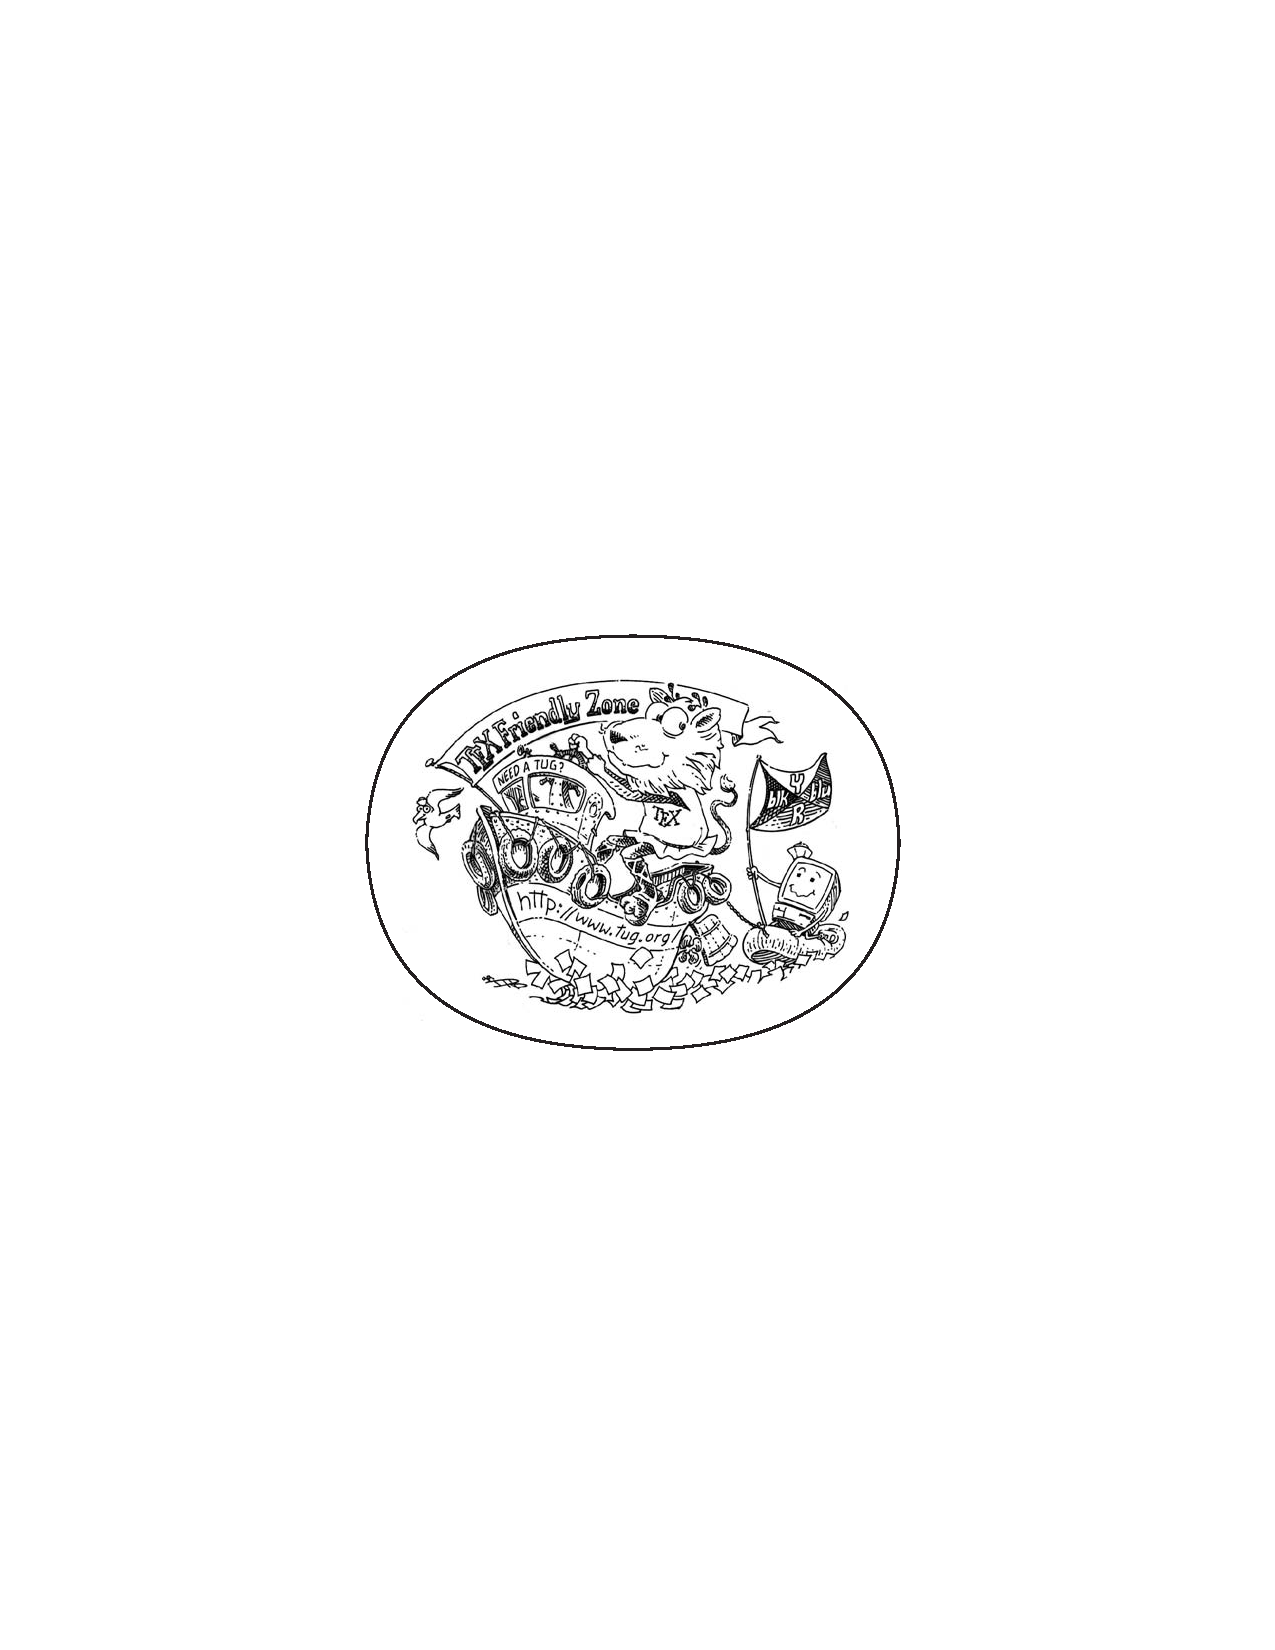
\includegraphics[width=6cm]{gfx/TFZsuperellipse_bw} \\ \medskip % Picture

Strugling for Happy Lives and Free Sprits\\ \medskip % Thesis subtitle
%\myDegree \\
%\myDepartment \\
%\myFaculty \\
%\myUni \\ \bigskip


\vfill

\end{center}
\end{addmargin}

\end{titlepage}

%% Back of the title page

\thispagestyle{empty}

\hfill

\vfill

\noindent\myName: \textit{\myTitle,} \mySubtitle, %\myDegree, 
\textcopyright\ \myTime

% You may wish to do something with the back of the title page, such as including your supervisors, location or time frame of the work. Below is an example of doing so although you may want to tweak it to your liking.

%\bigskip

%\noindent\spacedlowsmallcaps{Supervisors}: \\
%\myProf \\
%\myOtherProf \\ 
%\mySupervisor

%\medskip \\

%\noindent\spacedlowsmallcaps{Location}: \\
%\myLocation

%\medskip \\

%\noindent\spacedlowsmallcaps{Time Frame}: \\
%\myTime

%\cleardoublepage% Dedication

\thispagestyle{empty}
\refstepcounter{dummy}

\pdfbookmark[1]{Dedication}{Dedication} % Bookmark name visible in a PDF viewer

\vspace*{3cm}

\begin{center}
\emph{Ohana} means family. \\
Family means nobody gets left behind, or forgotten. \\ \medskip
--- Lilo \& Stitch    
\end{center}

\medskip

\begin{center}
Dedicated to the loving memory of Rudolf Miede. \\ \smallskip
1939\,--\,2005
\end{center}
%\cleardoublepage\include{FrontBackmatter/Foreword}
%\cleardoublepage% Abstract

\pdfbookmark[1]{Abstract}{Abstract} % Bookmark name visible in a PDF viewer

\begingroup
\let\clearpage\relax
\let\cleardoublepage\relax
\let\cleardoublepage\relax

\chapter*{Abstract} % Abstract name

Short summary of the contents\dots

\endgroup			

\vfill
%\cleardoublepage% Publications - a page listing research articles written using content in the thesis

\pdfbookmark[1]{Publications}{Publications} % Bookmark name visible in a PDF viewer

\chapter*{Publications} % Publications page text

Some ideas and figures have appeared previously in the following publications:

\bigskip

\noindent Put your publications from the thesis here. The packages \texttt{multibib} or \texttt{bibtopic} etc. can be used to handle multiple different bibliographies in your document.
%\cleardoublepage% Acknowledgements

\pdfbookmark[1]{Acknowledgements}{Acknowledgements} % Bookmark name visible in a PDF viewer

\begin{flushright}{\slshape    
We have seen that computer programming is an art, \\ 
because it applies accumulated knowledge to the world, \\ 
because it requires skill and ingenuity, and especially \\
because it produces objects of beauty.} \\ \medskip
--- \defcitealias{knuth:1974}{Donald E. Knuth}\citetalias{knuth:1974} \citep{knuth:1974}
\end{flushright}

\bigskip

%----------------------------------------------------------------------------------------

\begingroup

\let\clearpage\relax
\let\cleardoublepage\relax
\let\cleardoublepage\relax

\chapter*{Acknowledgements} % Acknowledgements section text

Put your acknowledgements here.\\

\noindent Many thanks to everybody who already sent me a postcard!\\

\noindent Regarding the typography and other help, many thanks go to Marco Kuhlmann, Philipp Lehman, Lothar Schlesier, Jim Young, Lorenzo Pantieri and Enrico Gregorio\footnote{Members of GuIT (Gruppo Italiano Utilizzatori di \TeX\ e \LaTeX )}, J\"org Sommer, Joachim K\"ostler, Daniel Gottschlag, Denis Aydin, Paride Legovini, Steffen Prochnow, Nicolas Repp, Hinrich Harms, Roland Winkler,  and the whole \LaTeX-community for support, ideas and some great software.

\bigskip

\noindent\emph{Regarding \mLyX}: The \mLyX\ port was intially done by
\emph{Nicholas Mariette} in March 2009 and continued by
\emph{Ivo Pletikosi\'c} in 2011. Thank you very much for your work and the contributions to the original style.

\endgroup
\pagestyle{scrheadings}
\cleardoublepage% Table of Contents - List of Tables/Figures/Listings and Acronyms

\refstepcounter{dummy}

\pdfbookmark[1]{\contentsname}{tableofcontents} % Bookmark name visible in a PDF viewer

\setcounter{tocdepth}{2} % Depth of sections to include in the table of contents - currently up to subsections

\setcounter{secnumdepth}{3} % Depth of sections to number in the text itself - currently up to subsubsections

\manualmark
\markboth{\spacedlowsmallcaps{\contentsname}}{\spacedlowsmallcaps{\contentsname}}
\tableofcontents 
\automark[section]{chapter}
\renewcommand{\chaptermark}[1]{\markboth{\spacedlowsmallcaps{#1}}{\spacedlowsmallcaps{#1}}}
\renewcommand{\sectionmark}[1]{\markright{\thesection\enspace\spacedlowsmallcaps{#1}}}

\clearpage

\begingroup 
\let\clearpage\relax
\let\cleardoublepage\relax
\let\cleardoublepage\relax

%----------------------------------------------------------------------------------------
%	List of Figures
%----------------------------------------------------------------------------------------

%\refstepcounter{dummy}
%\addcontentsline{toc}{chapter}{\listfigurename} % Uncomment if you would like the list of figures to appear in the table of contents
%\pdfbookmark[1]{\listfigurename}{lof} % Bookmark name visible in a PDF viewer

%\listoffigures

%\vspace*{8ex}
%\newpage

%----------------------------------------------------------------------------------------
%	List of Tables
%----------------------------------------------------------------------------------------

%\refstepcounter{dummy}
%\addcontentsline{toc}{chapter}{\listtablename} % Uncomment if you would like the list of tables to appear in the table of contents
%\pdfbookmark[1]{\listtablename}{lot} % Bookmark name visible in a PDF viewer

%\listoftables
        
%\vspace*{8ex}
%\newpage
    
%----------------------------------------------------------------------------------------
%	List of Listings
%---------------------------------------------------------------------------------------- 

%\refstepcounter{dummy}
%\addcontentsline{toc}{chapter}{\lstlistlistingname} % Uncomment if you would like the list of listings to appear in the table of contents
%\pdfbookmark[1]{\lstlistlistingname}{lol} % Bookmark name visible in a PDF viewer

%\lstlistoflistings 

%\vspace*{8ex}
%\newpage
       
%----------------------------------------------------------------------------------------
%	Acronyms
%----------------------------------------------------------------------------------------

%\refstepcounter{dummy}
%\addcontentsline{toc}{chapter}{Acronyms} % Uncomment if you would like the acronyms to appear in the table of contents
%\pdfbookmark[1]{Acronyms}{acronyms} % Bookmark name visible in a PDF viewer

%\markboth{\spacedlowsmallcaps{Acronyms}}{\spacedlowsmallcaps{Acronyms}}

%\chapter*{Acronyms}

%\begin{acronym}[UML]
%\acro{DRY}{Don't Repeat Yourself}
%\acro{API}{Application Programming Interface}
%\acro{UML}{Unified Modeling Language}
%\end{acronym}  
                   
\endgroup

\cleardoublepage

%********************************************************************
% Mainmatter
%*******************************************************
\pagenumbering{arabic}
%\setcounter{page}{90}
% use \cleardoublepage here to avoid problems with pdfbookmark
\cleardoublepage
\part{Spring 2014}
%
\chapter{April - 2012} % Chapter title

\label{ch:april:2012} % For referencing the chapter elsewhere, use \autoref{ch:introduction} 

%----------------------------------------------------------------------------------------
\section{Reading Game Theory}
Book name: {\it Fun and games, a text on game theory}

A game is being played whenever people interact with each other. What happens when people interact in {\bf a rational manner}

Those insects and plants whose genes programmed them to behave irrationally are now extinct.

We become distressed when confronted with {\bf circle reasoning}. But circle reasoning can not be evaded in considering strategic issues. 

Game theorists introduce their toy games with silly stories, which allow us to disengage our emotions from the problem.

\subsection{A example: One house, two bider}
Two bider: Horace and Maurice. 
The only way that Horace can be sure of keeping Maurice guessing, is by using a mixed strategy. What this means is that Horace should {\it \bf randomize} over the bids that it is sensible for him to make.

How should Horace randomize? For example, Never bid less than \$3 or more than \$ $3.5$.
If Horace seals \$b in his envelope,


{(\it 4.1 Payoffs)} Players act as though seeking to maximize the expected value of Von Neumann and Moregenstern utility function $u_i : \Omega \rightarrow \mathbb{R} $ defined on the set $\Omega$ of final outcomes of the game. Player $i$'s payoff at an outcome $\omega$ is then simply the Von Neumann and Moregenstern utility $u_i(\omega)$.
If the payoff $\phi$ includes a probability value, the game seems interesting.

{(\it 4.3 Matrices, 4.4 Vectors)} 

\subsection{2012-03-23}
rpc.rstatd is the dameon service of linux system information. The service collects such as CPU, system load and other information. If a client of rstat like rup or rsysinfo sends a request, the service will response the request. It is invoked by the system service xinetd. In addition, the service portmap provides the UDP output interface.  

\hfill {\tiny edited on 2012-04-29}

\section{Spell checking, Vim tips}
We should turn on the spell checking function in most of writing time.
\begin{enumerate}
\item Turn On:  \begin{center}\bf :set spell \end{center}
\item Turn Off:  \begin{center}\bf :set nospell \end{center}
\item Move the cursor to next wrong spelling:  \begin{center}\bf ]s \end{center}
\item Move the cursor to the previous wrong spelling:  \begin{center}\bf [s \end{center}
\item Add the user-defined word into the spell dictionary:  \begin{center}\bf zg \end{center}
\item Remove the user-defined word from the spell dictionary:  \begin{center}\bf uzg \end{center}
\item List all spelling recommendations about the wrong word:  \begin{center}\bf z= \end{center}
\item Set the spelling language:  \begin{center}\bf :set spelllang=en\_GB.UTF-8 \end{center}
\item Show the current spelling language:  \begin{center}\bf :echo \&spelllang  \end{center}
\end{enumerate}
\hfill {\tiny edited on 2012-04-27}

\section{Find and Replace, Vim tips}
\begin{enumerate}
\item The symbol {\bf \#} can be used for a separator, like the symbol {\bf /}. The following commands carry out the same functions.  
\begin{center}
35, 68 s/aaaa/bbbb/gc \\
35, 68 s\#aaaa\#bbbb\#gc
\end {center}
\end{enumerate}
\hfill {\tiny edited on 2012-04-27}

\section{Matrix, Matlab tips}
\label{sec:matlab}
\begin{enumerate}
\item Return every dimension of array $A$ in separate variables $m$ and $n$.  For example,
    $$[m,n] = \text{size}(A);$$
\item Return the $i$th row of array $A$ and the $j$th column of array $B$. For example,
    $$A(i,:);B(:,j);$$
\item {\bf Delete} the $i$th row of array $A$ and the $j$th column of array $B$. For example,
    $$A(i,:)=[\quad ]; B(:,j)=[\quad ];$$
\item Sum all values of elements in the $i$th column of array $A$. 
    $$\text{sum}(A(:,i))$$
\item Add a new row into array $A$ given that they have same column.
    $$A=[A;row];$$
\item Sum cumulatively the $j$th column of array $A$, 
    $$a = \text{cumsum}(A(:,j))$$
\item Clear the memory occupied by variables whose prefix is 'a', except the variable 'ab'.
    $$\text{clearvars a* -except ab};$$
\end{enumerate}
\hfill {\tiny edited on 2012-04-27}

\section{Moving smooth filter, Matlab}
When dealing with the data with plenty of samples, we use the tool, 'plot', to get the figure to show the trend of data.  If the interval of sampling is too small, the curve of samples seems to fluctuate drastically. It might cause the trouble that the trend not to be seen clearly. We use the tool, 'Moving Smooth filter' to handle the trouble.  
The function 
\begin{center}
$y$ = filter($b, a, x$)
\end{center}
creates the filtered data $y$ by processing the data in vector $x$ with the filter described by vectors $a$ and $b$.
The filter function is a general tapped delay-line filter, described by the difference equation, \autoref{eqn_moving_filter}.
\begin{align}
a(1)y(n) &= b(1)x(n) + b(2)x(n-1) + \cdots + b(N_b)x(n-N_b+1) \notag\\
& -a(2)y(n-1)- \cdots - a(N_a)y(n-Na+1)
\label{eqn_moving_filter}
\end{align}
\hfill {\tiny edited on 2012-04-29.}

\section{Plotting Figures, Default Values, Matlab}
Yesterday, I faced a problem about the default size of markers when I plotted a curve. After googled the content with the keywords 'default marker size', I got the information like this in the following:
For line objects, you can use
\begin{verbatim}
set(0,'DefaultLineMarkerSize',12);
set(0,'DefaultLineMarker','d');
set(0,'DefaultLineLineWidth', 2);
\end{verbatim}
Similarly, for axes objects, you can use these statements:
\begin{verbatim}
set(0,'DefaultAxesLineWidth', 2);
set(0,'DefaultAxesXGrid','on');
set(0,'DefaultAxesTickDir','out');
set(0,'DefaultAxesTickLength',[0.015 0.015]);
set(0,'DefaultAxesFontName','Arial')
\end{verbatim}
There are also two problems. One is that there are so many markers on curves that the figure seems unclear. I downloaded a tool called 'Nummarkers', which can set the number of makers shown on the curves. The other is that the gray figures with 'eps' format are not exported correctly. The tool 'ExportFig' can solve it. Note: the two tools can be download from the Matlab website.
\begin{verbatim}
h = plot(x,y1, x,y2);
nummarkers(h, 19, 1);

exportfig(h, strcat(main_dir_name,file_name,'.eps'), ... 
        'Format','eps', 'LockAxes', 1, 'Color', 'gray');
exportfig(h, strcat(main_dir_name,file_name,'.tif'), ...
        'Format','tiff', 'Resolution', 600, 'Color', 'rgb');
exportfig(h, strcat(main_dir_name,file_name,'.pdf'), ... 
    'Format', 'pdf', 'Color', 'rgb')
\end{verbatim}
\hfill {\tiny edited on 2012-04-29.}

\section{GSview}
GSview tool is used to view the EPS figures. The register codes are:
\begin{align*}
32411-26380\\
18963-21159\\
16417-30959
\end{align*}
\hfill {\tiny edited on 2012-04-29.}

\section{Beauty Face}
It is said that handsome faces have the two key ratio. The first one is the distance between two eyes to the distance between two ears. The second one is distance between eyes and mouth to the distance between chin and hair, shown in \autoref{fig:beauty_face}.
\begin{figure}
\begin{center}
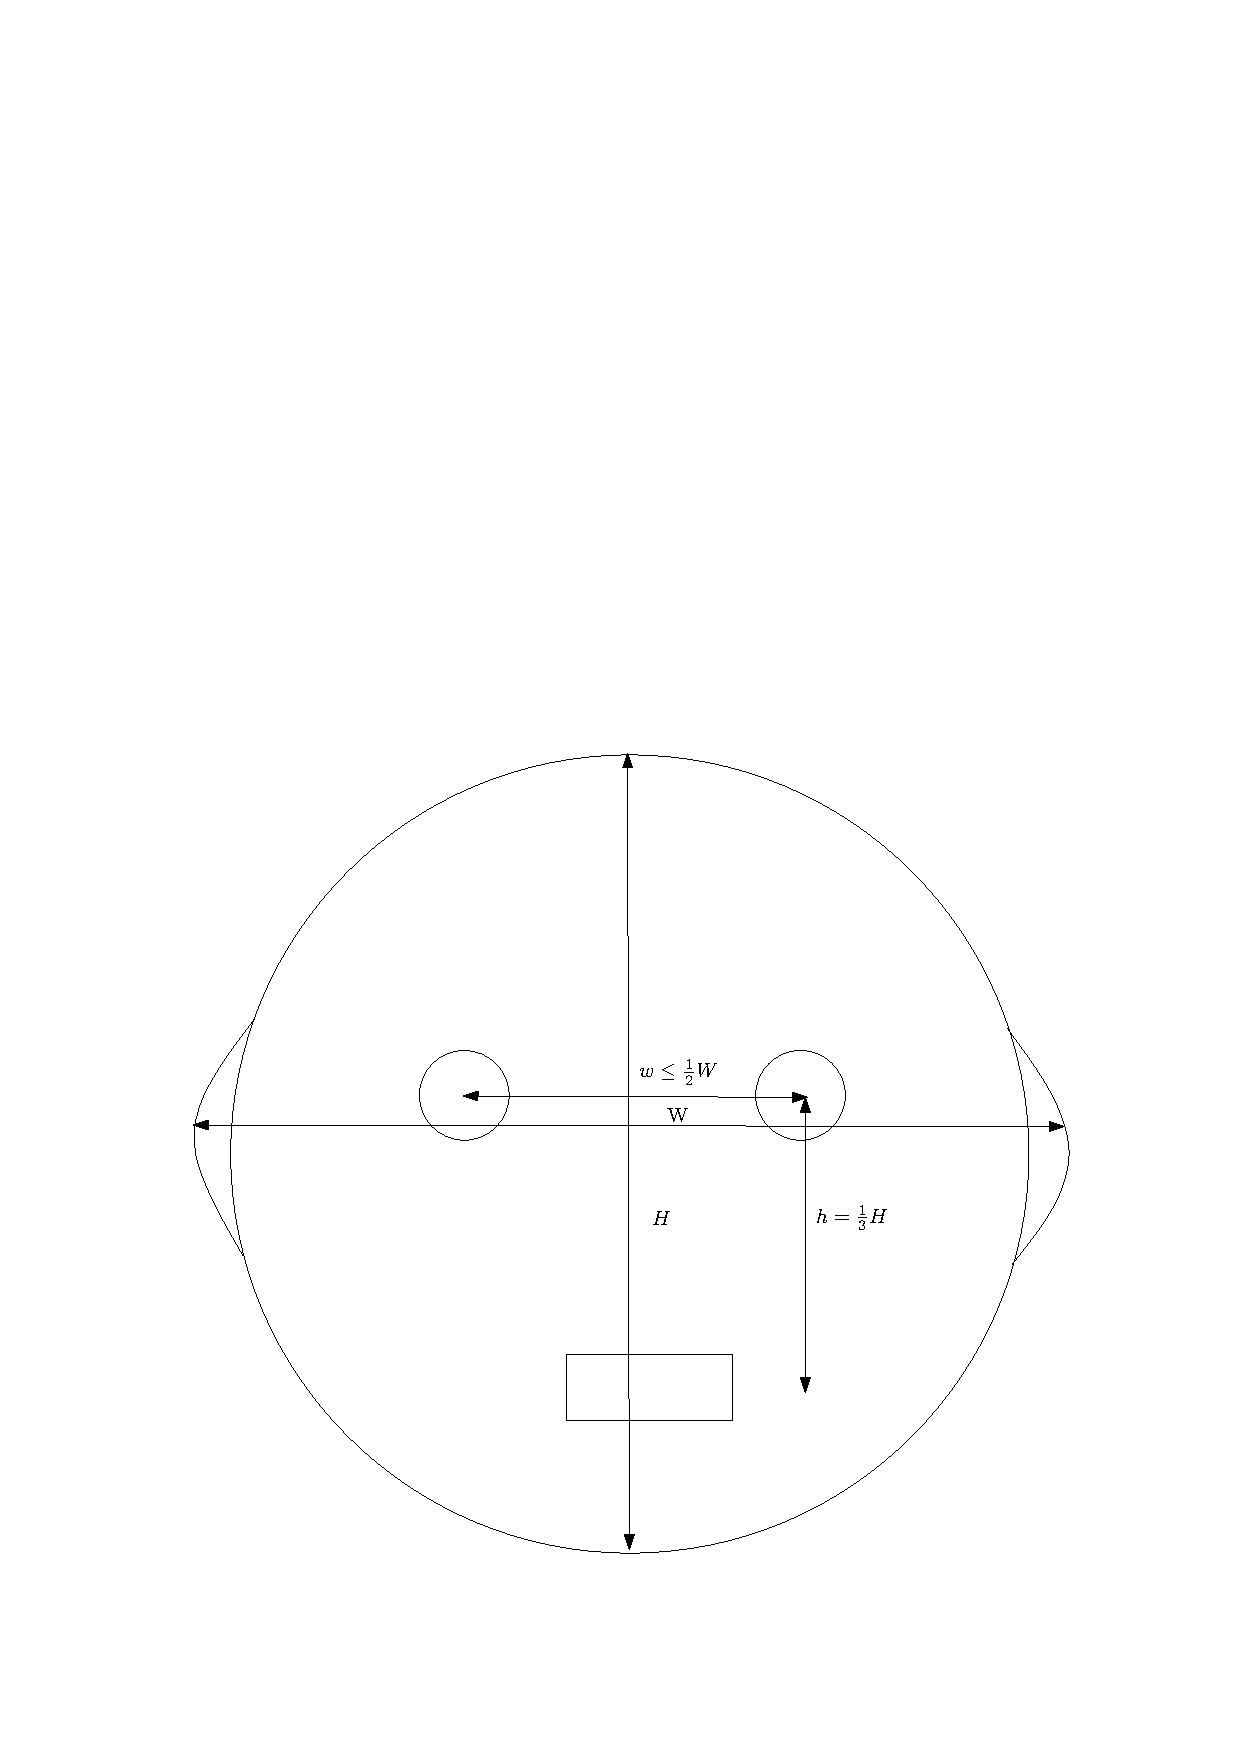
\includegraphics[width=.7\linewidth]{gfx/beauty_face}
\end{center}
\caption{The key ratios}
\label{fig:beauty_face}
\end{figure}
\hfill {\tiny edited on 2012-04-29.}

\section{Skype, China version}
If you make a call via the Skype-Tom Chinese version, you should add a symbol '*' before phone numbers. It looks like:
\begin{center}
*03733029531
\end{center}
\hfill {\tiny edited on 2012-04-30.}
\section{Git and Dropbox}
Today, I suddenly have a idea about backup of my important files. That method is to combine the Git and Drop-box. The Git system can deal with the version control. Drop-box automatically handles the backup operations on the remote server. The following steps are shown in detail here. We assume that the backup directory' name is "phd\_thesis", which includes several files, \texttt{"chapter01.doc"} and \texttt{"chapter01.bak"}. 
\begin{enumerate}
\item put a file named \texttt{'.gitignore'} into the root directory of 'phd\_thesis'. If we do not backup the file \texttt{'chapter01.bak'}, we insert its name into the \texttt{'.gitignore'} file. You have better add the names of ignored files into the file in advance. If the Git system have tracked the files, the complicated steps can remove them from the Git system.
\item Initialize Git on the working directory and files, like 
\begin{verbatim}
cd ~/phd_thesis
~/phd_thesis $ git init
~/phd_thesis $ git add .
~/phd_thesis $ git commit -m "first commit"
\end{verbatim}
\item Initialize Git on the Drop-box default directory, like
\begin{verbatim}
cd ~Dropbox/git
~/Dropbox/git $ git init --bare phd_thesis.git
\end{verbatim}
\item Sync the directories from local disk 'master' to drop-box 'phd\_thesis'.
\begin{verbatim}
~/phd_thesis $ git remote add phd_thesis 
                ~/Dropbox/git/phd_thesis.git
~/phd_thesis $ git push -u phd_thesis master
\end{verbatim}
\item Clone from the drop-box. 
\begin{verbatim}
Local clone:
    git clone  ~/Dropbox/git/phd_thesis.git
    git clone file://~/Dropbox/git/phd_thesis.git/chapter01.doc

Remote clone other computer's repository:
    git ssh://[user@]host.xz[:port]/path/to/repo.git/
    git git://host.xz[:port]/path/to/repo.git/
    git http[s]://host.xz[:port]/path/to/repo.git/
    git ftp[s]://host.xz[:port]/path/to/repo.git/
    git rsync://host.xz/path/to/repo.git/
\end{verbatim}
\end{enumerate}

\hfill {\tiny edited on 2012-04-30.}

\marginpar{Most people won't realize that writing is a craft. You have to take your appernticeship in it like anything else. \\
-Katherine Anne Porter}
%%%%%%%%%%%%%%%%%%%%%%%%%%%%%%%%%%%%%%%%%%%%%%%%

%\chapter{May - 2012} % Chapter title

\label{ch:may:2012} % For referencing the chapter elsewhere, use \autoref{ch:introduction} 

%----------------------------------------------------------------------------------------
\section{Reading Style Lessons}
\marginpar{Have something to say, and say it as clearly as you can. That is the only secret of style. \\
-Mathew Arnold}
\subsection{Clarity of an Article}
Someone criticizes you that your proses are not understandable. You  bewilder your readers because you can not organize your ideas coherently.  
People presume that the complex sentences with abstract and long words are equal to deep thinking. In fact, such sentences mean that you do not understand well what you write. So you have to hide the evidence from readers and even yourself.  
As a matter of fact, writing and thinking can help with each other.

\subsection{Correctness}
The rules are specific and the principles are abstract.
\subsubsection{Ruler}
There are three kinds of rulers, real rules, social rules and invented rules. The invented rules includes Folklore and Elegant.

The Folklore options are shown in the following:
\begin{enumerate}
\item The sentences began with \texttt{'And'} and \texttt{'But'} are acceptable.
\item \texttt{'Because'} and \texttt{'Since'}. The positions of two words are dependent on the prior knowledge of readers. The order of sentences are so important that we focus on it. We should put the familiar material in the first place and the strange ones later.
\item \texttt{'that'} and \texttt{'which'} in restrictive or non-restrictive clauses. Which is your choice depends on the emphasis of your idea. 
\item \texttt{'fewer'} and \texttt{'less'}. No one uses \texttt{fewer} with mass nouns (fewer dirt) but educated writers often use less with countable plural nouns (less resources).
\item \texttt{'since'} and \texttt{'while'}. The two words mean \texttt{because} and \texttt{although} if the clauses are more familiar to readers.  
\end{enumerate}
The Elegant options are:
\begin{enumerate}
\item {\bf Don't split infinitives ?} 
\begin{itemize}
\item[] $\surd$ to slightly conceal
\item[] $\surd$ to conceal slightly
\end{itemize}
\item{\bf whom or who?}
\begin{itemize}
\item []$\surd$ Who am I writing for?
\item []$\surd$ For whom am I writing?
\end{itemize}
If the relative clause modifies a noun and you can delete the relative pronoun and still make sense, the correct form is whom:
\begin{itemize}
\item []$\surd$ The committee chose someone whom they trusted.
\item []$\surd$ The committee chose someone [ ] they trusted.
\end{itemize}
If you cannot delete the \texttt{who/whom}, the correct form is \texttt{who}:
\begin{itemize}
\item []$\surd$ The committee chose someone {\bf who} earned their trust. 
\item []$\times$ The committee chose someone [ ] earned their trust.
\end{itemize}
Two exceptions:(1)you cannot delete \texttt{whom} when it begins a clause that is the object of a verb. In that case, you have to depend on the grammar of the clause:
\begin{itemize}
\item[]$\surd$ The committee decided \texttt{whom} they should choose.
\item[]$\surd$ The committee decided \texttt{who} was to be chosen.
\end{itemize}
(2)Always use whom when it is the object of a preposition:
\begin{itemize}
\item[]$\surd$ The committee choose someone in \texttt{whom} they had confidence. 
\end{itemize}

\end{enumerate}
\hfill {\tiny P.26, edited on 2012-05-01.}

\section{Crop PDF, Foxit Phantom}
What you do is: open the file that you want to crop, select menu, <Organize>-><Crop Pages...>, and setup the inch of margins and pages index. All things are down.
\hfill {\tiny  edited on 2012-05-02.}

\section{Reading Lessons of Clarity}
P.27\\
\begin{itemize}
\item Don't end a sentence with a preposition.
\item Use the singular with \texttt{'none'} and \texttt{'any'}.
\end{itemize}
Hobgoblins:
\begin{itemize}
\item Never use \texttt{'like'} for \texttt{'as'} or \texttt{'as if'}.\\
For example: \\
$\surd$ These operations failed like the earlier ones did.\\
$\surd$ These operations failed as the earlier ones did.
\item Don't use \texttt{'hopefully'} to mean \texttt{'I hope'}.\\
For example:\\
$\surd$ Hopefully, it will not rain.\\
$\surd$ I hope that it will not rain.
\item Don't use \texttt{'finalize'} to mean \texttt{'finish'} or \texttt{'complete'}.
\item Don't use \texttt{'impact'} as a verb, but as a noun.
\item Don't modify absolute words such as \texttt{ perfect, unique, final complete} with \texttt{ very, more
    quite}, and so on.
\end{itemize}

Some Words That attract Special Attention\\
aggravate, anticipate, anxious, cohort, comprise, continuous, disinterested, enormity, fortuitous, fulsome, 
notorious.

P.38\\
Two principles:
\begin{itemize}
\item Its main characters are subjects of verbs.
\item Those verbs express specific actions.
\end{itemize}
P.42\\
Readers will think your writing is dense if you use lots of abstract nouns, especially those derived from verbs and adjectives,
nouns ending in -tion, -ment, -ence, and so on, especially when you make those abstract nouns the subjects of verbs.

A noun derived from a verb or adjective has a technical name: nominalization. The word illustrates its meaning: When we nominalize nominalize, we create the nomialization nominalization.

\section{Multiple clipboard, Vim}
The multiple clipboard is provided by Vim. The function can make us work more efficiently.  The buffer of clipboard has its name, which looks like ("b). The symbol means a buffer named \texttt{b}. If you want to save the current line into the buffer b, press {\bf "byy}. After that, you paste the content in buffer b into wherever you assign. The instruction is: {\bf"bp}. 

\section{Clarity in English Writing}
\marginpar{You write your prose for your readers.}
Choosing between Active and Passive P.65
\begin{enumerate}
\item Must your readers know who is responsible for the action?
\item Would the active or passive verb help your readers move more smoothly from one sentence to the next?
\item Would the active or passive give readers a more consistent and appropriate point of view?
Some writers switch from one character to another for no apparent reason. You should avoid this.
\end{enumerate}

When academic writers do use the first person, however, they use it in certain ways. There are two kinds:
\begin{itemize}
\item One kind refers to research activities: \texttt{study, investigate, examine, observe, use}. Those verbs are usually in the passive voice: 
\emph{ The subjects were observed $\ldots$} .
\item The other kind of verb refers not to the subject matter or the research, but to the writer's own writing and thinking: \emph{cite, show, inquire.}
These verbs are often active and in the first person: \emph{We will show $\ldots$ }. 
\end{itemize}
\hfill {\tiny  edited on 2012-05-02.}
\section{IPE draw tool, Image Conversion}
IPE is an excellent draw tool, which can create high quality vector figures. For example, it can generate the file with extension .eps or .pdf. These figures must be converted into bitmap format (.png) if you want to insert them into Microsoft Word. The conversion command line is:
\begin{verbatim}
Usage: iperender [ -svg | -png ] [ -page <page> ]
    [ -view <view> ] [ -resolution <dpi> ] infile outfile
Iperender saves a single page of the Ipe document in some formats.
 -page       : page to save (default 1).
 -view       : view to save (default 1).
 -resolution : resolution for png format (default 72.0 ppi).
\end{verbatim}

Or you want to export figures with PDF format.
\begin{verbatim}
Usage: ipetoipe ( -xml | -eps | -pdf ) <options> infile [ outfile ]
Ipetoipe converts between the different Ipe file formats.
 -export      : output contains no Ipe markup.
 -pages <n-m> : export only these pages (implies -export).
 -view <p-v>  : export only this view (implies -export).
 -lastview    : export only last view of each page (implies -export).
 -runlatex    : run Latex even for XML output.
 -nocolor     : avoid any color commands in EPS output.
 -nozip:      : do not compress PDF streams.
 -styleupdate : update style sheets.
\end{verbatim}
\hfill {\tiny  edited on 2012-05-04.}
\section{Latex, Table, Caption}
Sometimes, you need place the caption of a table below its content. You do it by the commands.
\begin{verbatim}
\begin{table}
\begin{tabular}
\end{tabular}
\caption{Example}
\end{table}
\end{verbatim}
\begin{table}[h]
\centering
\begin{tabular}{ccc}
\toprule
1 & 2 &3\\
\midrule
1 & 2 &3\\
1 & 2 &3\\
1 & 2 &3\\
\bottomrule
\end{tabular}
\caption{Example}
\end{table}
\hfill {\tiny  edited on 2012-05-04.}

\section{IEEE, Latex template, figure}
The IEEEtran document class will only center figure captions in Conference Mode, i.e. document class option "conference" is set.
(See also IEEEtrans documentation "How to Use the IEEEtran LATEX Class", page 2: "Conference Mode Details: Conference mode makes a number of significant changes to the way IEEEtran behaves.
\hfill{\tiny edited on 2012-05-04.}

\section{Latex, Fourier Macro package}
The package makes the fonts more graceful so that it is worth trying.
\begin{verbatim}
\usepackage{fourier}
\usepackage[OT1]{fontenc} %if there are CJK characters
\end{verbatim}
\hfill{\tiny edited on 2012-05-04.}
\section{Clarity in English Writing}
\begin{enumerate}
\item The terms active and passive, are ambiguous, because they can refer not only to those two grammatical constructions,
but to how a sentence make you feel.
\item Most readers want the subjects of verbs to name the main characters in a story 
and those main characters to be flesh and blood.
\item P.62 If you are in favour of something, you support it and think that it is good thing.
\item Reconstructing absent characters and remove nominlaization or abstract words.
\item P.79 We can achieve clarity just by mapping characters and actions onto subjects and verbs.
\item P.80 The last four words introduce an important character who is the subject of next sentence.
\item P.82 Begin sentences with information familiar to your readers. It includes a few words in the last sentence and what readers always know.
\item End sentences with information the readers can not anticipate. 
\item this, these, that, those, another, such, second, more
\item What is the difference between cohesive and coherence? The characters must belong to only one thing, one topic.
\end{enumerate}
\hfill {\tiny  edited on 2012-05-04.}
\section{Vim, words count}
\begin{center}
\bf press <g>, and then <ctrl>+<g>
\end{center}
\hfill {\tiny  edited on 2012-05-04.}
\section{EBOOK, Reading}
I download some books for further reading. They are:
\begin{enumerate}
\item \emph{English Grammar workbook for dummies}
\item \emph{Beyond feelings: A guide to critical thinking}
\item \emph{Using social Theory: Thinking through Research}
\end{enumerate}
\hfill {\tiny  edited on 2012-05-05.}
%
\section{Collins Dictionary, icon meaning}
\begin{itemize}
\item D, Dictionary
\item T, Thesaurus, same meaning words
\item U, Usage
\item G, Grammar
\item W, Word bank
\end{itemize}
\hfill {\tiny  edited on 2012-05-08.}
%
\section{Pip, Python Package Management}
\begin{enumerate}
\item Install a package, \begin{center} \$pip install <package-name> \\\$pip install <package-name>==<version>\end{center}
\item Update a package, \begin{center} \$pip install -upgrade <package-name> >= <version> (if you do not provide the version number, the latest version will be obtained.)\end{center}
\item Remove a package, \begin{center} \$pip uninstall <package-name> \end{center}
\end{enumerate}
\hfill {\tiny  edited on 2012-05-08.}
%
\section{Word 2007, Aurora, Equation, Update}
If you want to update all equations, select the menu <aurora, properties> from the ribbon of word menu and change some properties. The system will update the all equations in the document. And there are some bugs when you use the equation with index numbers, which cause the word system collapse.
\hfill {\tiny  edited on 2012-05-08.}
%
\section{Wrap lines, Vim}
We can set the limit of a line with the command such as 'set tw=$500$'. If you do not set a limit, just 'set tw=$0$'.
\hfill {\tiny  edited on 2012-05-09.}
%
\section{Xelatex, Fontspec Package}
Xelatex can use the package fontspec to assign a specific font as main font. (Tips: update l3kernel fontspec packages).
\begin{verbatim}
\documentclass[11pt,a4paper]{article}
\usepackage{fontspec}
\setmainfont{STSong}
% Chinese Line Wrapper
\XeTeXlinebreaklocale "zh"
\XeTeXlinebreakskip = 0pt plus 1pt
% Skip Two Chinese Characters
\makeatletter
\let\@afterindentfalse\@afterindenttrue
\@afterindenttrue
\makeatother
\setlength{\parindent}{2em}

\begin{document}
Chinese Characters
{\fontspec{STSong} Chinese Characters}
\end{document}
\end{verbatim}
\hfill {\tiny  edited on 2012-05-11.}
%
\section{Caption, Label, Latex}
Today, I confront a problem. The cross referencing number of all tables are wrongly linked to the section number in my article . After googling the web, the solution is found :
Put caption clause before label clause, such like:
\begin{verbatim}
\caption{Simulations Table} \label{tb:sim_res}
\end{verbatim}
\hfill {\tiny  edited on 2012-05-11.}
%
\section{Noun, Verb, Modifier, VIM}
Vim system has its unique grammar system. In short, it includes Noun, Verb, and Modifier. The position commands, like 'j', '0', '\$' and so on, are nouns. Verb are 'd'(delete), 'c'(change), 'y'(yank,copy) and 'v'(visual). Modifiers are 'i'(inside), 'a'(around), 't'(untill) and 'f'(find). 
\begin{center}
\bf Noun $+$ Verb $+$ Modifier $+$ Objects
\end{center}
Pay more attention to the modifier 'i' and 'a'.
\hfill {\tiny  edited on 2012-05-13.}
%
\section{log system, glog, google log}
Google log system is a excelent log system. The basic step is:
\begin{enumerate}
\item install, \begin{verbatim} ./configure; make; make install \end{verbatim}
\item add a function for sending email
\begin{itemize}
\item Install SendEmail; 
\begin{verbatim}apt-get install sendmail; 
apt-get install libio-socket-ssl-perl;
sendEmail -f username@foo.com -t destination@foo.com 
    -cc carboncopy@foo.com 
    -u "Message title" 
    -m "The body of the message" 
    -s smtp.foo.com:25 
    -xu username 
    -xp password \end{verbatim} 
\item Modify the logging.cc:1504
\begin{verbatim}string cmd = FLAGS_logmailer 
    + " -f sender.drumtm@gmail.com 
    -s smtp.gmail.com:25 
    -o tls=auto 
    -xu sender.drumtm 
    -xp 5hRZeEQGzn1asmL" 
    + " -u " + "\"" + subject + "\"" 
    + " -m " +"\"" + body +"\"" 
    + " -t " + dest; 
    \end{verbatim} 
\item Modify the logging.cc: 135 
\begin{verbatim}
GLOG_DEFINE_string(logmailer, "/usr/bin/sendEmail", 
    "Mailer used to send logging email"); 
\end{verbatim}
\end{itemize} 
\item re-install
\begin{verbatim} ./configure; make; make install \end{verbatim}
\item modify the cpp file
\begin{verbatim}
#include <glog/logging.h>
main()
{
    google::SetLogDestination(google::INFO,("./log.txt"));
    google::InitGoogleLogging("");
    google::SendEmail("to@gmail.com", "subject", "body");
    LOG(INFO) << "Found ";
    google::ShutdownGoogleLogging();
}\end{verbatim}
\end{enumerate}
\hfill {\tiny  edited on 2012-05-13.}
%
\section{ncurses, TTY, GDB}
\begin{enumerate}
\item Prepare two xterm windows, use the command {\bf tty} to identify the name of tty.
\item Redirect the screen information (such as printf)to tty1.
\begin{verbatim}
$GDB> tty /dev/tty1
\end{verbatim}
\end{enumerate}
\hfill {\tiny  edited on 2012-05-13.}
%
\section{Curses, Program}
Today, I study the program using a package called n-curses. 
Because I hope I can do a skeleton program for future codings. 
The skeleton program will include three parts: recording the log on local disk, sending email to developers and displaying a concise user interface. 
First two of them will be implemented by Google logging system. 
\par The final one will be done by the n-curses.
I did several trials and understood the mechanism of n-curses. 
The window in curses systems, in fact, is a block of memory, saving the responding data structures.
What we do is to display it on the terminal screen at the proper time.
The display routines are called {\bf wrefresh(WINDOWS*) }, which puts the characters that changes just now if the specific window are not active.
Thus, if you want totally clean refresh operations, first of all is to activate the windows by {\bf touchwin(WINDOW*)}.
Some examples are shown in the following:
\begin{verbatim}
switch (n) {
   case 1:
       touchwin(fix_win);
       wrefresh(fix_win);
       break;
   case 2:
       touchwin(scroll_win);
       wrefresh(scroll_win);
       break;
   case 0:
       touchwin(stdscr);
       wrefresh(stdscr);
       break;
   default:
       touchwin(stdscr);
       wrefresh(stdscr);
       break;
}
napms(500);
\end{verbatim}
\hfill {\tiny  edited on 2012-05-14.}
%
\section{Align, Program, C}
Left align:
\begin{verbatim}
printf("%-40s", str);
\end{verbatim}
Right align:
\begin{verbatim}
printf("%40s", str);
\end{verbatim}
\hfill {\tiny  edited on 2012-05-14.}
%
\section{Data Exchange, Json}
JSON (Java Script Object Notation) is a text format for data exchange. 
It is simpler than XML format.
JSON includes Object, Array, String, and Number Types.
Perhaps, I could use the format for future coding.
\hfill {\tiny  edited on 2012-05-15.}
%
\section{Separate, UI and Code}
In the last two days, I consider some problems for future coding. 
The problems consist of Logging and front-end user interface (UI) design. 
This morning, I am suddenly aware of the importance of loose connections between front-end UI and back-end programs. 
The back-end programs should be independent of the UI. 
They ought be connected only by a data structure like JSON.
\hfill {\tiny  edited on 2012-05-15.}
%
\section{UNIX, Command, Find}
Unix program principle: One Tool One work. 
Thus, you will combine the two commands with together.
\begin{verbatim}
find   /opt   -name '.svn'|xargs rm -r
\end{verbatim}
\hfill {\tiny  edited on 2012-05-17.}
%
\section{Ubuntu, Install, GCC}
\begin{verbatim}
$ sudo apt-get install build-essential
$ sudo apt-get install linux-headers-$(uname -r)
\end{verbatim}
\hfill {\tiny  edited on 2012-05-18.}
%
\section{Python, Html, QT}
I have been searching a Python library that handles html files with CSS. Today, I find my solution, QtWebKit, from QT library family.
\begin{verbatim}
import os, sys

import winsound
import time
# Import PySide classes
from PySide.QtCore import *
from PySide.QtGui import *
from PySide.QtWebKit import *

# Go through the dir "html"
class DisplayHtml(QWebView):
    def __init__(self, html_file_list):
        QWebView.__init__(self)
        self.counter = 1
        self.html_file_list = html_file_list
        self.file_num = len(self.html_file_list)       
        #self.load(QUrl("c:/tmp/my_codes/get_english_words/html/2012_03_07/woo.html") )
        self.show()
        self.timer = QTimer(self)
        self.connect(self.timer, SIGNAL("timeout()"), self.LoadHtml)
        self.timer.start(2500)
        self.stop_flag = 0
    def keyPressEvent(self, e):
        if e.key() == Qt.Key_Escape:
            self.close()
        if e.key() == Qt.Key_Space:
            self.stop_flag = self.stop_flag^1 
            if self.stop_flag == 1:
                self.timer.stop()
            else:
                self.timer.start()

    def LoadHtml(self):
        if self.counter < self.file_num:
                html_file = self.html_file_list[self.counter]
                html_file = html_file.replace('\\', r'/')

                self.setWindowTitle(html_file)
                self.setUrl(html_file)

                wav_file = html_file.replace('html','wav')
                ret = os.access(wav_file, os.F_OK)
                if True==ret:
                    wav = winsound.PlaySound(wav_file, winsound.SND_FILENAME)
                self.counter = self.counter + 1
        else:
            self.counter = 0 
            self.html_file_list.reverse()


def listdir_fullpath(d):
    return [os.path.join(d, f) for f in os.listdir(d)]


# Enter Qt application main loop
#print html_date_dir

# Display the Web file
g_pwd = os.getcwd()
g_today_string = time.strftime("%Y_%m_%d", time.localtime(time.time())); 
        
print "Enter a directory name (eg. %s):" %(g_today_string)
date_dir = raw_input(">")
date_dir = date_dir.strip()

if len(date_dir)<2:
    html_date_dir = g_pwd + '/html/'+ g_today_string +'/'
    wav_date_dir = g_pwd + '/wav/'+ g_today_string +'/'
else:
    date_dir = time.strftime("%Y_%m_", time.localtime(time.time()))+ date_dir
    html_date_dir = g_pwd + '/html/'+ date_dir +'/'
    wav_date_dir = g_pwd + '/wav/'+ date_dir +'/'

html_file_list = listdir_fullpath(html_date_dir)
# Create a Qt application
if __name__=='__main__':
    app = QApplication(sys.argv);
    brower = DisplayHtml(html_file_list);
    sys.exit(app.exec_());

\end{verbatim}
\hfill {\tiny  edited on 2012-05-27.}
%
\section{GDB, Assembly}
\begin{verbatim}
(gdb) set disassembly-flavor intel
(gdb) set disassemble-next-line on
(gdb) b *0x08048431
(gdb) ni
(gdb) disass main
(gdb) si
\end{verbatim}
\hfill {\tiny  edited on 2012-05-28.}
%
\section{Prey, Email, Phone, SMS}
Yesterday, the unhappy events happened. 
I have to monitor the following things that will happen next.
I enabled the 'Prey' to collect the screen-shot and forwarded the notice mail from G-mail to to 139 email.
If any emails arrive, the 139 Email system will notice me via SMS. That is it.
\hfill {\tiny  edited on 2012-05-29.}
%
 
%% Chapter 1
\chapter{June - 2012}
\section{Vim, unfold}
If you expand all unfold text, press 'ZR' in the normal mode.
\par \hfill {\tiny  edited on 2012-06-02.}
%----------------------------------------------------------------------------------------

%%%%%%%%%%%%%%%%%%%%%%%%%%%%%%%%%%%%%%%%%%%%%%%%

 
%\chapter{August - 2012} % Chapter title
\label{ch:aug:2012} % For referencing the chapter elsewhere, use \autoref{ch:introduction} 

%----------------------------------------------------------------------------------------

\section{Reading, Take a step back}
In the past years, Aaron Swartz was the decider, tasked with making the best selection from the options life presented.
He could play with this friend or that one, go to this college or that one, take this job offer or the other one.

Instead of just picking the best option, Aaron try to invent new ones. Instead of just avoiding the stuff that bugs him, should he start making plans to fix them.

It is a big change for him psychologically, which influence me much more. I see the positive and active attitude of his facing tough life from the article. Just as he said, he is charting his destiny, instead of following some track. 


\url{http://www.aaronsw.com/weblog/stepback}
\hfill {\tiny  edited on 2012-08-20.}

\section{Reading, Batman Begins}
The article written by Aaron Swartz is about the movie "batman". He told us briefly the story about the history of Batman. In practice, the history is how the two sides, organized criminal groups and the rich, keep their power balanced. The power hold by either of sides make all people, both the rich and the poor, suffer from the unbalanced world. Even if the rich who seems  on behalf of the positive side holds stronger power, the common people who live in the world will still suffer. It sounds ridiculous, which is true for us in the real world.
\hfill {\tiny  edited on 2012-08-24.}

%\chapter{September - 2012} % Chapter title
\label{ch:sep:2012} % For referencing the chapter elsewhere, use \autoref{ch:introduction} 

%----------------------------------------------------------------------------------------

\section{SublimeText 2, Crack}
Although I want to pay the software 'SublimeText', the price is too expensive for me.
I have to search the crack over the Internet, the crack solution is:
\begin{enumerate}
\item  Use the vim to open the programe file as binary format;
\item  Find the string "3542 4535 3039 4333 3342 3032 3031 3131";
\item  Change '3342' to '3242';
\item  Then, using the following license to register.
\end{enumerate}
\begin{comment}
\end{comment}
\begin{verbatim}
-----BEGIN LICENSE-----
Zhiwei
Unlimited User License
EA7E-27304
295F06AD49A222300142F52385B79017
0EBC472E766824A3E764A77BEE8905AB
532EA109E190C3E75483FF14D0010DFA
5F532494C59E830CCE5002A0BE9110EC
0B2AC29AB5BEAAA3242124FD2B99A2CE
F443912E3A653CDE9195B7C15D5ED807
F7C3904D5473C89529796E723C79C019
3809B28DBBF4E34CAC38938A8389B925
-----END LICENSE-----
\end{verbatim}
\hfill {\tiny edited on 2012-09-23}

\section{Vim, Edit, Binary File}
Vim can edit a binary file easier than the editor "Emacs". 
You need the tool 'xxd' to dump a file from binary format to text format.
After editing, you use 'xxd' to revert the file format into binary. 
For example,

\begin{verbatim}
vi -b bin_file_name
:%!xxd
....
editing something
....
:%!xxd -r
:wq
\end{verbatim}
\hfill {\tiny edited on 2012-09-23}

\section{Vim Crash, Input Method, Chinese Character Directory Name}
The VIM, SublimeText2 and Notepad++ crashed after I installed a new WB98 word bank for JiDianWB.
I wondered why and how the installation made this happen. 
Finally, I found the reason.
The reason is that the directory name of the new word bank is spelled as Chinese characters.
Since my computer OS is the Windows 7 English version, the input method manager seems not to handle the Chinese Directory Name well.
The solution is very simple, changing the directory name from Chinese characters to English letters.
\hfill {\tiny  edited on 2012-09-17}

\section{Python, Urlopen}
Today, the Website of dictionary, "iCiba", blocked my access through Python scripts after my looking up several words. 
After several trials, I found the solution: If using the standard usage for HTTP protocols, the problem can be solved.
The codes in the following:

\par From 
\begin{verbatim}
    try:
        page = urllib2.urlopen(g_collins_url+word)
    except urllib2.HTTPError, e:
        print g_collins_url, e.code
        return False
    soup = BeautifulSoup(page)

\end{verbatim}

\par To
\begin{verbatim}
    try:
        req = urllib2.Request(g_collins_url+word)
        response = urllib2.urlopen(req)
    except urllib2.HTTPError, e:
        print g_collins_url, e.code
        return False

    page = response.read()
    soup = BeautifulSoup(page)
\end{verbatim}
\hfill {\tiny  edited on 2012-09-19.}
%
\section{Combine Picture for Longman Words}
Since the LongmanCN dictionary splits one word picture into several frames,
I have to make a small program script to combine them, like this:
\begin{verbatim}
  if match:
        fp = open(str(word_dir+file),'rb')
#       print file;
        old_image = Image.open(fp)
        y = old_image.size[1];
        new_image.paste(old_image, (x_index, y_index));
        fp.close();

        x_index = 0;
        y_index = y_index + y;
        os.remove(word_dir+file)
\end{verbatim}
It is noted that the picture file should be closed if you remove or delete it. 
Since the IMage library does not support the method 'close',
you have to take an alternative way to handle this.
\hfill {\tiny  edited on 2012-09-19.}


%%%%%%%%%%%%%%%%%%%%%%%%%%%%%%%%%%%%%%%%%%%%%%%%%%%%%%%%%

%\chapter{November - 2012} % Chapter title
\label{ch:nov:2012} % For referencing the chapter elsewhere, use \autoref{ch:introduction}

%----------------------------------------------------------------------------------------------------

\section{SublimeText 2, disappear}
Today, I found the window of the program `SublimeText' disappeared. 
The window did not appear although I tried many times to restore it.
After a while, I found the reason. 
The multi-screen causes the SublimeText not to set its windows correctly. 
I can press the keys `<Win> + <Left Arrow>' to move it to the current screen.
\hfill {\tiny  edited on 2012-11-09.}

\section{Redhat, RHEL 6.2}
\subsection{Change, password, root}
In order to get familiar with Redhat 6.2, I installed it in the virtual machine by means of the Vmware.
However, I forget the password of the user 'root'.
After surfing the Internet, I found the solution. 
It can be reset through boot loader 'grub'.
After you see the boot menu, press 'e' to edit the boot item, like "kernel /vmlinuz-2. ro root".
You just append the word " single" on the item, and press 'b' to boot the machine.
You can login the linux OS as the user 'root'.
The command 'passwd' can change the password of 'root' without the old password.

\subsection{GUI from X windows to Multiuser}
You should edit the file '/etc/inittab', changing '5' into '3'.
For example, 'id:5:' to 'id:3:'.
After the system boots, the GUI interface will be changed into terminal window style.

\subsection{Configure, IP, eth0}
You edit the file '/etc/sysconfig/network-scripts/ifcfg-eth0' to set up the network interface of eth0.
For example, 
Device=eth0
BOOTPROTO=none
ONBOOT=yes
NETMASK=255.255.255.0
IPADDR=10.0.1.6
USERCTL=no

\url{https://access.redhat.com/knowledge/docs/en-US/Red_Hat_Enterprise_Linux/6/html/Deployment_Guide/s1-networkscripts-interfaces.html }
\hfill {\tiny  edited on 2012-11-13.}

\section{Samba, RHEL}
In order to restore the work environment, I install the samba server which can share files with the Windows OS clients.

The steps is shown in the following:
\begin{enumerate}[(1)]
\item Install samba server software in the RHEL 6.2.  you should execute the command as the user root: rpm -ivh samba-3.5.10-114.el6.i686.rpm
\item After installation, run the command 'rpm -q samba' to verify the samba server.
\item Go to the directory '/etc/samba', and find three files: smbusers, smb.conf, and lmhosts. For the file lmhosts, add the windows OS computer IP and name. For example,
\begin{verbatim}
        192.168.122.1 yanzw-PC
\end{verbatim}
For the file smbusers, add the user name. For example,
\begin{verbatim}
        username=lian
\end{verbatim}. 
For the file smb.conf, add the shared directory. For exmple, 
\begin{verbatim}
        [shared]
        path = /home/shared
        writeable = yes
        browseable = yes
        read only = No
        guest ok = Yes
        public = Yes
        valid users = yzw lian
        create mask = 0666
        directory mask = 0777
\end{verbatim}
\item run the commands:
\begin{verbatim}
    mkdir shared
    chmod a+w shared
    chcon -t samba_share_t shared
    useradd -c "PGSql Developer" -d /home/lian -s /sbin/nologin lian
    smbpasswd -a lian
   /sbin/service smb restart
   /sbin/service nmb restart
\end{verbatim}
\end{enumerate}
\hfill {\tiny  edited on 2012-11-15.}

\section{shared library, RHEL 6.2}
The command 'ldconfig' can refresh the library cache. 
If your program does not find the library, you should add your required library path into the system library path, modifying the file '/etc/ld.so.conf'.
\hfill {\tiny  edited on 2012-11-14.}

\section{PostgreSQL, Reading}
\subsection{Database Infransture}
The PostgreSQL runs as the mode 'Client/Server'. 
The program called "postgres" is the server process, which executes all commands of clients. It supports concurrent connections using 'fork()'.
The client programs submit their requests to the process 'postgres', and display the responses from the server.
\subsection{users}
PostgreSQL users are different from the Unix users.
You should add the specifical user for the database.
The server must be run by the PostgreSQL user account and not by root or any other user.
\subsection{Source, Installation}
You run the following commands as the user 'root'.
\begin{verbatim}
./configure
gmake
su
gmake install
\end{verbatim}

\subsection{Add user, directory of data}
You run the following commands as the user 'root'.
\begin{verbatim}
adduser postgres
mkdir /usr/local/pgsql/data
chown postgres /usr/local/pgsql/data
\end{verbatim}

\subsection{Initilize DB server, run DB server}
You run the following commands as the user 'root'.
\begin{verbatim}
su - postgres
/usr/local/pgsql/bin/initdb -D /usr/local/pgsql/data
/usr/local/pgsql/bin/postgres -D /usr/local/pgsql/data >logfile 2>&1 &
\end{verbatim}

\subsection{Create database example}
\begin{verbatim}
/usr/local/pgsql/bin/createdb test
/usr/local/pgsql/bin/psql test
=# select current_date;
=# \q
\end{verbatim}

\subsection{Template database}
There are two template databases, 'postgres' and 'template1'.

\subsection{Out of memory}
The memory parameters can be changed in the file '/etc/sysctl.conf'

\subsection{authentication}
pg\_hba.conf means host-based authentication.

\hfill {\tiny  edited on 2012-11-16.}


\section{Document, Writing, Rules}
\begin{enumerate}[(1)]
    \item All information should be recored in English in the jotting files.
    The jotting files are located in directory 
    \begin{verbatim}
    'c:\user\yanzw\desktop\my_jotting\'
    \end{verbatim}
    \item You should write the detail in English as possible as you can.
\end{enumerate}
\hfill {\tiny  edited on 2012-11-17.}


\section{Glog, SendMail}
\subsection{SendMail}
The SendMail is a Email program that send email via outside smtp server from a command line.
The command line options is shown in Fig. \ref{fig:send:mail:command}
You can download the program from 
\url{http://caspian.dotconf.net/menu/Software/SendEmail/}.

\begin{figure}[htbp]
\centering
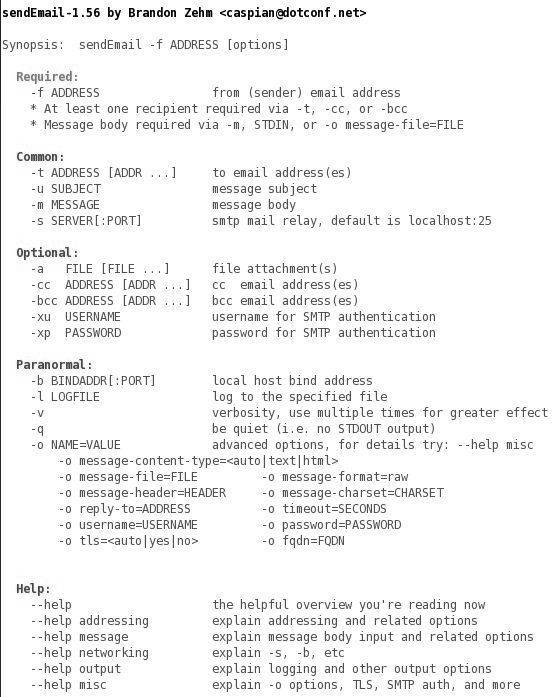
\includegraphics[width=0.95\textwidth]{./Chapters/pictures/sendEmail.jpg}
\caption{SendEmail}
\label{fig:send:mail:command}
\end{figure}
\hfill {\tiny  edited on 2012-11-09.}

\section{Venture lab, brainstorming}
\subsection{Room}
First, there has to be room for people walk around.
Second, there are space enough on a whiteboard to capture all the ideas.
\subsection{Participants}
The people should have different points of view and expertise on the topic.
They get together to collect all possibilities.
The policy of the size of group is 'two-pizza teams'.
\subsection{topic}
The question you ask is the frame into which the solution will fall.
\subsection{How to start a brainstorming session}
Maybe you can start with a seemingly silly prompt. For example, 'how would you design eyeglasses if we didn't have ears?'.
\subsection{Rules of brainstorming}
The participants aren't allowed to criticize ideas.
The key is to embrace all ideas that generated and to work with them for a while.
You must not evaluate ideas as they are generated.
It is also important to encourage wild and crazy ideas.
Even though they may seem strange, there may be a gem hidden inside.
Students can come up with the worst ideas they can during a brainstorming session.
When people are asked to generate bad ideas, they defer judgement and push beyond obvious solutions.
\subsection{Process of brainstorming}
One approach is to remove the most obvious solutions from the pool of possibilities, so that you have to come up with something new or strange.
Someone comes up with an idea, and several people build on it for a short time.
Then you jump to a new approach. 
The dance could be called 'build, build, build, Jump!'.
\subsection{Capture ideas}
Everyone has a pen and paper or sticky notes.
\subsection{Time}
It do not exceed more than one hour.
Maybe it is ten to fifteen minutes.
\subsection{Decision}
Everyone votes for all the ideas.

\subsection{Final step}
Take photos of all the ideas, make notes about the best ones, and save all the materials that can be saved.
As time goes by, some of the ideas that seem impractical might look promising.

\hfill {\tiny  edited on 2012-11-20.}

\section{RHEL 6.2 CDROM}
Question: I found the CDROM was not mounted automatically if I changed the GUI interface to Bash interface.
Solution: 
\begin{enumerate}[(1)]
    \item Create the directory: \begin{verbatim} mkdir \cdrom \end{verbatim} 
    \item Execute the command: \begin{verbatim} mount \dev\cdrom \cdrom \end{verbatim}
\end{enumerate}

\hfill {\tiny  edited on 2012-11-28.}


%\chapter{December - 2012} % Chapter title
\label{ch:dec:2012} % For referencing the chapter elsewhere, use \autoref{ch:introduction}

%----------------------------------------------------------------------------------------------------

\section{Git, learn}
Today, we applied for a commercial version on the GitHub website.
I have to relearn the commands about git.
\begin{enumerate}[(1)]
\item push the codes to the remote repository.
\begin{verbatim}
git push https://github.com/ssurui/openssl-test-demo master
User name for 'https://github.com': ZhiweiYAN
Password for 'https://ZhiweiYAN@github.com' : 
\end{verbatim}
\end{enumerate}
\hfill {\tiny  edited on 2012-12-25.}


\chapter[January - 2014]{January - 2014} % Chapter title

\label{ch:jan:2014} % For referencing the chapter elsewhere, use \autoref{ch:introduction} 

%----------------------------------------------------------------------------------------
\section{Remove comments from files in C}
You use the tool {\it gcc} to remove the comments in files.
\begin{verbatim}
gcc -fpreprocessed -dD -E test.c
\end{verbatim}

\hfill {\tiny edited on2014-03-05.}

\section{Big data  are we making a big mistake}
\marginpar {\tiny edited on 2014-04-02.}
Big data: are we making a big mistake?
By Tim Harford

\url{http://www.ft.com/cms/s/2/21a6e7d8-b479-11e3-a09a-00144feabdc0.html#axzz2xS1VXiUc}


\chapter{Feb - 2014} % Chapter title

\label{ch:feb:2014} % For referencing the chapter elsewhere, use \autoref{ch:introduction} 

%----------------------------------------------------------------------------------------
\section{Handle Excel files in C}
Perhaps, we begin to handle Microsoft Excel files in C.
We do the search over the Internet.
There are several packages or libraries that can be used.
\begin{enumerate}
\item xlsLIB, C++/C library to construct Excel .xls files in code. 
Detail in \url{http://sourceforge.net/projects/xlslib/files/}
\item Office (2007) Open XML File Formats. Detail in \url{http://msdn.microsoft.com/en-us/library/aa338205.aspx}
\item CSV formats. The format do not handle Chinese characters very well, 
since it includes the information of encoding in itself.
\end{enumerate}
The last two methods are recommended strongly. 

\section{20 Years of Web Development}
I read the ariticle {\it 20 Years of Web Development}, written by Reuven M. Lerner, 
a well-known columnist of Linux Journal.
The idea from the article make me feel something inside, same as the author.

If I can not get my fix of e-mail, or blogs, or newspapers or Hacker News,
I feel cut off from the rest of the world.
I'd like to take the opportunity to look at where Web technologies have come from,
and where they're going.

\subsection{In the Beginning}
In the beginning, the Web was static.
A Web brower requested a document from the server.
Instead, the server could lie to the browser,
creating a document on the fly, by executing a program.
The Web servers invoke external programs in a 'cgi-bin' directory.
The 'cgi' programs could be written in C and shell, 
later, in Perl and Tcl in those days.

For example, MIT students put their newspapers on the Web in 1993,
and made it possible for people to search through the newspaper's archives.

In 1995, no one really thought the web programming as serious software development.
At that time, applications were serious desktop software. 
I began to understand where the Web was head when you learned about relational databases
and understand how powerful Web applications could be when connected to a powerful,
flexible system for storing and retrieving data.
DB ranking list is at \url{http://db-engines.com/en/ranking}.

And at that point, the browser could be the beginning of a new platform for applications.
[PPTs also turn the bullets scheme into words-scheme.]
Nowadays, the vision has turned into a reality.
\par\hfill {\tiny edited on 2014-02-27}

\subsection{Libraries and Frameworks}
It did not take long before Web development really began to take off.
The growth of the Web happened at about the same time that the term {\it open source} was coined.
Open-source operating systems and languages - in those days,
Perl, Python and PHP - grew in popularity, both because they were free of charge
and because they offered enormous numbers of standardized, debugged and highly useful
libraries.


%%%%%%%%%%%%%%%%%%%%%%%%%%%%%%%%%%%%%%%%%%%%%%%%


\chapter[March - 2014]{March - 2014} % Chapter title

\label{ch:mar:2014} % For referencing the chapter elsewhere, use \autoref{ch:introduction} 

%----------------------------------------------------------------------------------------
\section{Remove comments from files in C}
You use the tool {\it gcc} to remove the comments in files.
\begin{verbatim}
gcc -fpreprocessed -dD -E test.c
\end{verbatim}

\hfill {\tiny edited on2014-03-05.}

\section{Color Scheme in Borland C++}
The backgroud is blue, 0, 0, 168, 0000A8.
The text is yellow, FFFF44, 255,255,68

\marginpar{Most people won't realize that writing is a craft. You have to take your appernticeship in it like anything else. \\
-Katherine Anne Porter}
%%%%%%%%%%%%%%%%%%%%%%%%%%%%%%%%%%%%%%%%%%%%%%%%


\chapter[April - 2014]{April - 2014} % Chapter title

\label{ch:apr:2014} % For referencing the chapter elsewhere, use \autoref{ch:introduction} 

%----------------------------------------------------------------------------------------
\section{Big data  are we making a big mistake}

Big data: are we making a big mistake?
By Tim Harford

\url{http://www.ft.com/cms/s/2/21a6e7d8-b479-11e3-a09a-00144feabdc0.html#axzz2xS1VXiUc}

Sometimes, {\bf Big Data analysis} produces uncannily accurate results; They are cheap to collect relative to their size and they are a messy collage of datapoints collected for disparate purposes and
they can be updated in real time. 

\begin{enumerate}
\item cheap to collect
\item collage of datapoints
\item disparate purposes
\item update in real time
\end{enumerate}

With enough data, "the numbers speak for themselves".

As our communication leisure and commerce have moved to the internet and the internet has moved into our phones, our cars and even our glasses or watches,  life can be recorded and quantified in a way that would have been hard to imagine just a decade ago.
There are a lot of small data problems that occur in big data, says Spiegelhalter.  "They don't disappear because you've got lots of the stuff. They get worse."


We seek new ways to understand our lives.
Figuring out what causes what is hard (impossible" some say).
If you have no idea what is behind a correlation, you have no idea what might cause that correlation to break down. 

Statisticians have spent the past 200 years figuring out what traps lie in wait when we try to understand the world through data. 
They cared  about correlation rather than causation.
When it comes to data, size isn't everything.

US-based Twitter users were disproportionately young  urban or suburban and black.
There must always be a question about who and what is missing" especially with a messy pile of found data.
Twitter users are not representative of the population as a whole.
Who cares about causation or sampling bias" though" when there is money to be made?
We found data contain systematic biases and it takes careful thought to spot and correct for those biases. 

There are two issues: sample error and sample bias. The larger the sample, the smaller the margin of error (sample error). 
The sample bias is more dangerous, because the sample is not randomly 
choosen at all. 
You should find an unbias sample. Find the detail in {\it Number sense}, wroten by Kaiser Fung.
Another bias example is about the iPhone app, {\it Boston Street Bump}.
You should find data contain systematic biases and it takes careful thought to
spot and correct for those biases.

{\bf Multiple-comparisons problem: }
We observed pattern could have emerged at random, we call that pattern "statistically significant".
"Why Most Published Research Findings Are False"
There are a few cases in which analysis of very large data sets has worked miracles, like
Google Translate.

Big data do not solve the problem that has obsessed statisticians and scientists for centuries: the problem of insight , of inferring what is going on, and figuring out how we might intervene to change a system for the better.  To use big data to produce such answers will require large strides in statistical methods.
"But nobody wants 'data'. What they want are the answers."
Many contrary results are languishing in desk drawers because they just didn't seem interesting enough to publish. 

{\bf{"Big data"}} has arrived but big insights have not. The challenge now is to solve new problems and gain new answers -- without making the same old statistical mistakes on a grander scale than ever.
As for the idea that "with enough data" the numbers speak for themselves" -- that seems hopelessly naive in data sets where spurious patterns vastly outnumber genuine discoveries.


\hfill {\tiny edited on 2014-04-02.}

%%%%%%%%%%%%%%%%%%%%%%%%%%%%%%%%%%%%%%%%%%%%%%%%

\chapter[May - 2014]{May - 2014} % Chapter title

\label{ch:may:2014} % For referencing the chapter elsewhere, use \autoref{ch:introduction} 

%----------------------------------------------------------------------------------------
\section{Stop Wasting Users' Time}
Title: Stop Wasting Users' Time BY , 
URL:\url{http://www.smashingmagazine.com/2014/04/25/stop-wasting-users-time/}

What is the single most precious commodity in Westen society? Money? Status?
I would argue it is time.

\begin{enumerate}
    \item CAPTCHA: The Ultimate Time-Waster, any system that forces the user to prove they are human.
    \item Why Are Password So Complicated: Can't we come up with a better solution than an arcane mix of uppercase, numbers and symbols? complexicity and long phrase.
    \item Don't Make Users Correct 'Their' Mistakes in Forms. Sometimes we even waste the user's time when we are trying to help them. Forms are paticularly painful on touchscreens.
    \item Pay Special Attention To Repetitive Tasks. For that matter, a more robust solution to 'Remember me' functionality would be nice, so that users are, in fact, remembered.
    \item Help Users Process Our Content Faster: We can also make our content a lot more scannable, with better use of headings, pullout quotes and lists.
\end{enumerate}

\marginpar {\tiny 2014-05-05.}


%\include{Chapters/Chapter01}
\cleardoublepage
%%\ctparttext{You can put some informational part preamble text here. 
%Illo principalmente su nos. Non message \emph{occidental} angloromanic
%da. Debitas effortio simplificate sia se, auxiliar summarios da que,
%se avantiate publicationes via. Pan in terra summarios, capital
%interlingua se que. Al via multo esser specimen, campo responder que
%da. Le usate medical addresses pro, europa origine sanctificate nos se.}
%\part{The Showcase}
%\include{Chapters/Chapter02}
%%\addtocontents{toc}{\protect\clearpage} % <--- just debug stuff, ignore
%\include{Chapters/Chapter03}
%%\include{multiToC} % <--- just debug stuff, ignore for your documents
%% ********************************************************************
%% Backmatter
%%*******************************************************
%\appendix
%\cleardoublepage
%\part{Appendix}
%\include{Chapters/Chapter0A}
%%********************************************************************
%% Other Stuff in the Back
%%*******************************************************
%\cleardoublepage% Bibliography

\label{app:bibliography} % Reference the bibliography elsewhere with \autoref{app:bibliography}

\manualmark
\markboth{\spacedlowsmallcaps{\bibname}}{\spacedlowsmallcaps{\bibname}} 
\refstepcounter{dummy}

\addtocontents{toc}{\protect\vspace{\beforebibskip}} % Place the bibliography slightly below the rest of the document content in the table of contents
\addcontentsline{toc}{chapter}{\tocEntry{\bibname}}

\bibliographystyle{plainnat}

\bibliography{Bibliography}
%\cleardoublepage% Colophon (a brief description of publication or production notes relevant to the edition)

\pagestyle{empty}

\hfill

\vfill

\pdfbookmark[0]{Colophon}{colophon}

\section*{Colophon}

This document was typeset using the typographical look-and-feel \texttt{classicthesis} developed by Andr\'e Miede. The style was inspired by Robert Bringhurst's seminal book on typography ``\emph{The Elements of Typographic Style}''. \texttt{classicthesis} is available for both \LaTeX\ and \mLyX: 

\begin{center}
\url{http://code.google.com/p/classicthesis/}
\end{center}

\noindent Happy users of \texttt{classicthesis} usually send a real postcard to the author, a collection of postcards received so far is featured here: 

\begin{center}
\url{http://postcards.miede.de/}
\end{center}
 
\bigskip

\noindent\finalVersionString
%\cleardoublepage% Declaration

\refstepcounter{dummy}
\pdfbookmark[0]{Declaration}{declaration} % Bookmark name visible in a PDF viewer

\chapter*{Declaration} % Declaration section text

\thispagestyle{empty}

Put your declaration here.
\bigskip
 
\noindent\textit{\myLocation, \myTime}

\smallskip

\begin{flushright}
\begin{tabular}{m{5cm}}
\\ \hline
\centering\myName, \today \\
\end{tabular}
\end{flushright}

% ********************************************************************
% Game Over: Restore, Restart, or Quit?
%*******************************************************
\end{document}
% ********************************************************************
